\documentclass[aspectratio=169,11pt]{beamer}
% =====================================================================
%  Le Collé — thème de présentation (même palette et mêmes notations que la fiche)
% =====================================================================
\usepackage[utf8]{inputenc}
\usepackage[T1]{fontenc}
\usepackage[sc]{mathpazo}
\usepackage[scaled=0.92]{helvet}
\usefonttheme{professionalfonts}
\usepackage{amsmath,amssymb,mathrsfs,stmaryrd}
\usepackage{microtype}
\usepackage{booktabs,array,multicol}
\usepackage[most]{tcolorbox}
\usepackage{tikz,pgfplots}
\usetikzlibrary{arrows.meta,calc,positioning,decorations.pathreplacing,shapes.misc}
\pgfplotsset{compat=1.17,trig format plots=rad}
\usepackage{tkz-tab}

% ---------- palette (identique à la fiche) ----------
\definecolor{Ink}{HTML}{1C2533}\definecolor{Bleu}{HTML}{1F3A5F}\definecolor{BleuMoyen}{HTML}{4A6A8F}
\definecolor{BleuClair}{HTML}{9DB2C9}\definecolor{Fond}{HTML}{F2F4F7}\definecolor{Ocre}{HTML}{B07A26}
\definecolor{Brique}{HTML}{A23B2A}\definecolor{Gris}{HTML}{5E6672}\definecolor{Filet}{HTML}{C5CCD6}
\definecolor{Vert}{HTML}{2E6B4F}

% ---------- notations (identiques à la fiche) ----------
\newcommand{\K}{\mathbb{K}}\newcommand{\R}{\mathbb{R}}\newcommand{\C}{\mathbb{C}}\newcommand{\Z}{\mathbb{Z}}
\newcommand{\Mn}[1]{\mathcal{M}_{n}(#1)}\newcommand{\rg}{\operatorname{rg}}\newcommand{\vect}{\operatorname{Vect}}
\newcommand{\Mat}{\operatorname{Mat}}\newcommand{\Id}{\operatorname{Id}}\newcommand{\com}{\operatorname{com}}
\newcommand{\vv}[1]{\overrightarrow{#1}}\newcommand{\ve}[1]{\vec{#1}}
\newcommand{\dt}[1]{\left|\begin{matrix}#1\end{matrix}\right|}
\DeclareRobustCommand{\HP}{{\sffamily\bfseries\scriptsize\textcolor{Brique}{[HP]}}}

% ---------- réglages beamer ----------
\setbeamertemplate{navigation symbols}{}
\setbeamersize{text margin left=0.85cm,text margin right=0.85cm}
\setbeamercolor{normal text}{fg=Ink,bg=white}
\setbeamercolor{structure}{fg=Bleu}
\setbeamercolor{alerted text}{fg=Brique}
\setbeamerfont{alerted text}{series=\bfseries}
\setbeamertemplate{itemize item}{\raisebox{0.15em}{\textcolor{Ocre}{\rule{0.38em}{0.38em}}}}
\setbeamertemplate{itemize subitem}{\textcolor{BleuMoyen}{\scriptsize\textbullet}}
\setbeamertemplate{enumerate item}{\textcolor{Bleu}{\sffamily\bfseries\insertenumlabel.}}
\setlength{\leftmargini}{1.2em}
\setbeamertemplate{blocks}[default]

% numéro de la partie courante, rappelé dans le titre et le pied de page (renvoi à la fiche)
\def\fichesec{}\def\chapnom{}
\newcommand{\chapitre}[1]{\def\chapnom{#1}}

\setbeamertemplate{frametitle}{%
  \vskip0.28cm
  \ifx\fichesec\empty\else
    \tikz[baseline=(b.base)]\node[fill=Ocre,text=white,font=\sffamily\bfseries\scriptsize,inner sep=2.5pt,rounded corners=1pt](b){\fichesec};\hspace{0.45em}%
  \fi
  {\color{Bleu}\sffamily\bfseries\Large\insertframetitle}\par
  \vskip0.06cm{\color{Filet}\rule{\linewidth}{0.5pt}}\vskip-0.2cm}

\setbeamertemplate{footline}{%
  \hbox to\paperwidth{%
    \hspace*{0.85cm}{\scriptsize\sffamily\color{Gris}Le Collé\ \ \textcolor{Filet}{|}\ \ \chapnom}\hfill
    {\scriptsize\sffamily\color{Gris}\ifx\fichesec\empty\else fiche \textbf{\color{Ocre}§\fichesec}\quad\fi\insertframenumber}\hspace*{0.85cm}}%
  \vskip0.18cm
  \hbox{\begin{tikzpicture}
    \fill[Fond] (0,0) rectangle (\paperwidth,2.2pt);
    \pgfmathsetmacro\prog{min(\insertframenumber/max(\inserttotalframenumber,1),1)}
    \fill[Ocre] (0,0) rectangle ({\prog*\paperwidth},2.2pt);
  \end{tikzpicture}}}

% ---------- encadrés : même code couleur que la fiche ----------
\tcbset{sb/.style={enhanced,arc=1pt,boxrule=0pt,left=6pt,right=6pt,top=3pt,bottom=3pt,before skip=0.14cm,after skip=0.14cm,
  fontupper=\normalsize\raggedright}}
\newcommand{\etiq}[2]{{\sffamily\bfseries\scriptsize\color{#1}\MakeUppercase{#2}}\par\vspace{2pt}}
\newtcolorbox{DEF}[1][Définition]{sb,colback=white,borderline west={2pt}{0pt}{Bleu},before upper={\etiq{Bleu}{#1}}}
\newtcolorbox{PROP}[1][Propriété]{sb,colback=Fond,borderline west={3pt}{0pt}{Bleu},before upper={\etiq{Bleu}{#1}}}
\newtcolorbox{FORM}[1][Formule]{sb,colback=white,colframe=BleuMoyen,boxrule=0.6pt,before upper={\etiq{BleuMoyen}{#1}}}
\newtcolorbox{METH}[1]{sb,colback=white,borderline north={1pt}{0pt}{Bleu},borderline south={1pt}{0pt}{Bleu},
  before upper={{\sffamily\bfseries\scriptsize\colorbox{Bleu}{\color{white}MÉTHODE}\ \color{Bleu}#1}\par\vspace{3pt}}}
\newtcolorbox{PIEGE}[1][Piège]{sb,colback=Brique!6,borderline west={2pt}{0pt}{Brique},before upper={\etiq{Brique}{#1}}}
\newtcolorbox{ASTU}[1][Astuce]{sb,colback=Ocre!8,borderline west={2pt}{0pt}{Ocre},before upper={\etiq{Ocre}{#1}}}
\newtcolorbox{HPBOX}{sb,colback=white,borderline west={2pt}{0pt}{Brique},before upper={\etiq{Brique}{Hors programme}}}
\newtcolorbox{ATOI}[1][À toi]{sb,colback=Vert!6,borderline west={2pt}{0pt}{Vert},before upper={\etiq{Vert}{#1}}}
\newtcolorbox{RETENIR}{sb,colback=Bleu!5,colframe=Bleu,boxrule=0.8pt,left=8pt,
  before upper={\etiq{Bleu}{À retenir}}}
\newtcolorbox{EX}[1][Exemple]{sb,colback=white,colframe=Filet,boxrule=0.5pt,before upper={\etiq{Gris}{#1}}}

% complément pédagogique absent du livre : étiquette pointillée
\DeclareRobustCommand{\ajout}{\tikz[baseline=(a.base)]\node[draw=Gris,dashed,text=Gris,font=\sffamily\scriptsize,inner sep=2pt,rounded corners=1pt](a){complément hors livre};}
\newcommand{\livre}[1]{{\sffamily\scriptsize\color{Gris}[livre #1]}}
\newcommand{\rep}[1]{\textcolor{Vert}{#1}}% réponse attendue de l'élève

% ---------- styles de figures (identiques au livre) ----------
\pgfplotsset{courbe/.style={axis lines=middle,axis equal image,
  axis line style={Gris,-{Stealth[length=4pt]}},
  xlabel={$x$},ylabel={$y$},ticklabel style={font=\scriptsize\sffamily,color=Gris},
  every axis x label/.style={at={(ticklabel* cs:1)},anchor=west,font=\small},
  every axis y label/.style={at={(ticklabel* cs:1)},anchor=south,font=\small},
  samples=200,smooth}}
\pgfplotsset{mini/.style={axis lines=middle,axis line style={Filet},xtick=\empty,ytick=\empty,width=3.9cm,height=3.9cm,
  xmin=-1.15,xmax=1.15,ymin=-1.15,ymax=1.15,title style={font=\footnotesize\sffamily,yshift=-0.1cm},samples=100}}
\tikzset{arcetude/.style={Bleu,line width=1.25pt},
         reste/.style={BleuClair,line width=1pt},
         tgte/.style={Ocre,line width=1pt},
         asy/.style={Gris,dashed,line width=0.7pt},
         pt/.style={circle,fill=Ink,inner sep=1.3pt},
         >={Stealth[length=5pt]}}

% ---------- diapositives de partie ----------
% \partie{num}{titre}{question guide}{liste des parties du chapitre via \rm}
\newcommand{\rmitem}[2]{\def\tmp{#1}%
  \ifx\tmp\fichesec{\color{Bleu}\bfseries #1\quad #2}\else{\color{Gris!70}#1\quad #2}\fi\par\vspace{2pt}}
\newcommand{\partie}[4]{%
  \def\fichesec{#1}\section{#2}%
  \begin{frame}[plain]
  \begin{tikzpicture}[remember picture,overlay]
    \fill[Bleu] (current page.north west) rectangle ([xshift=6.3cm]current page.south west);
    \node[anchor=north west,text=white,font=\sffamily\bfseries\fontsize{40}{40}\selectfont] at ([xshift=0.8cm,yshift=-1.2cm]current page.north west) {#1};
    \node[anchor=north west,text width=4.8cm,align=left,text=white,font=\sffamily\bfseries\Large] at ([xshift=0.8cm,yshift=-2.9cm]current page.north west) {\hyphenpenalty=10000\exhyphenpenalty=10000 #2\par};
    \node[anchor=south west,text width=4.8cm,text=white!75!Bleu,font=\sffamily\scriptsize] at ([xshift=0.8cm,yshift=0.6cm]current page.south west) {\chapnom\\fiche \textbf{§#1}};
  \end{tikzpicture}
  \hspace*{5.5cm}\begin{minipage}{8.4cm}
  {\sffamily\scriptsize\color{Ocre}\bfseries LA QUESTION}\par\vspace{2pt}
  {\large #3}\par\vspace{0.7cm}
  {\sffamily\scriptsize\color{Gris}\bfseries DANS CE CHAPITRE}\par\vspace{4pt}
  {\sffamily\small #4}
  \end{minipage}
  \end{frame}}


% ---------- exercices en séance : énoncé sur une diapositive, correction sur la suivante ----------
\newcommand{\badgeexo}[1]{\tikz[baseline=(e.base)]\node[fill=Vert,text=white,font=\sffamily\bfseries\scriptsize,inner sep=2.5pt,rounded corners=1pt](e){EXERCICE #1};\hspace{0.4em}}
\newcommand{\badgecor}[1]{\tikz[baseline=(e.base)]\node[draw=Vert,line width=0.8pt,text=Vert,font=\sffamily\bfseries\scriptsize,inner sep=2.2pt,rounded corners=1pt](e){CORRECTION #1};\hspace{0.4em}}
\newtcolorbox{ENONCE}[1][]{sb,colback=Vert!6,borderline west={3pt}{0pt}{Vert},left=9pt,top=5pt,bottom=5pt,
  before upper={{\sffamily\bfseries\scriptsize\color{Vert}À TOI\ifx\relax#1\relax\else\ \ ·\ \ \MakeUppercase{#1}\fi}\par\vspace{4pt}}}
\newtcolorbox{INDICE}{sb,colback=white,colframe=Vert!60,boxrule=0.5pt,before upper={\etiq{Vert}{Indice (si besoin)}}}
\newtcolorbox{RAIS}[1][Le raisonnement]{sb,colback=Vert!5,borderline west={2pt}{0pt}{Vert},before upper={\etiq{Vert}{#1}}}
\newtcolorbox{OUTIL}{sb,colback=Fond,borderline west={2pt}{0pt}{Bleu},before upper={\etiq{Bleu}{Propriété ou méthode utilisée}}}
\newcommand{\etape}[1]{{\sffamily\bfseries\footnotesize\color{Vert}#1}\ }
\newcommand{\objectif}[1]{\par\vspace{2pt}{\footnotesize\sffamily\color{Gris}Objectif : #1}}

\title{Le Collé --- Déterminants et courbes paramétrées}

\begin{document}

% ---------------------------------------------------------------- titre
\begin{frame}[plain]
\begin{tikzpicture}[remember picture,overlay]
  \fill[Bleu] (current page.north west) rectangle (current page.south east);
  \node[anchor=north west,text=white!70!Bleu,font=\sffamily\scriptsize] at ([xshift=1cm,yshift=-1.2cm]current page.north west)
    {LE COLLÉ\ \ ·\ \ MATHÉMATIQUES PT\ \ ·\ \ SUPPORT DE SÉANCE};
  \node[anchor=north west,text=white,font=\sffamily\bfseries\fontsize{26}{30}\selectfont,text width=13cm] at ([xshift=1cm,yshift=-2.1cm]current page.north west)
    {Déterminants\\ Courbes paramétrées planes};
  \fill[Ocre] ([xshift=1cm,yshift=-4.6cm]current page.north west) rectangle ([xshift=4cm,yshift=-4.65cm]current page.north west);
  \node[anchor=north west,text=white!80!Bleu,font=\normalsize,text width=12cm] at ([xshift=1cm,yshift=-5cm]current page.north west)
    {Présentation pour expliquer ; la \textbf{fiche de référence} pour travailler et réviser.\\
     Mêmes parties (§1.1 à §2.7), mêmes notations, mêmes énoncés.};
\end{tikzpicture}
\end{frame}

% ---------------------------------------------------------------- mode d'emploi
\begin{frame}{Comment lire ce support}
\vspace{-0.15cm}
\begin{columns}[T]
\column{0.48\textwidth}
\begin{DEF}vocabulaire à connaître\end{DEF}\vspace{-9pt}
\begin{PROP}[Propriété / théorème]énoncé précis, avec ses hypothèses\end{PROP}\vspace{-9pt}
\begin{FORM}formule et conditions d'emploi\end{FORM}\vspace{-9pt}
\begin{METH}{}démarche à suivre, étape par étape\end{METH}
\column{0.48\textwidth}
\begin{PIEGE}erreur classique à éviter\end{PIEGE}\vspace{-9pt}
\begin{ASTU}technique qui fait gagner du temps\end{ASTU}\vspace{-9pt}
\begin{ATOI}question ou exercice ; correction à la diapositive suivante\end{ATOI}\vspace{-9pt}
\begin{RETENIR}l'essentiel d'une partie\end{RETENIR}
\end{columns}
{\footnotesize Même code couleur que la fiche. \ajout{} : ajout absent du livre. \ \HP{} : hors programme.
\ Le numéro ocre \tikz[baseline=(b.base)]\node[fill=Ocre,text=white,font=\sffamily\bfseries\scriptsize,inner sep=2pt](b){1.2};
\ renvoie à la partie de la fiche.}
\end{frame}

% ---------------------------------------------------------------- plan
\begin{frame}{Plan et séances}
\begin{columns}[T]
\column{0.48\textwidth}
{\sffamily\bfseries\color{Bleu}Chapitre 1 --- Déterminants}\par\vspace{4pt}
\small
1.1\quad Dimensions 2 et 3\\
1.2\quad Définition et règles de calcul\\
1.3\quad Propriétés globales, endomorphismes\\
1.4\quad Géométrie\\
1.5\quad Quelle méthode pour quel déterminant ?\\
1.6\quad Techniques d'ordre $n$\\
{\color{Gris}1.7\quad Résultats des TD (fiche)}
\column{0.48\textwidth}
{\sffamily\bfseries\color{Bleu}Chapitre 2 --- Courbes paramétrées}\par\vspace{4pt}
\small
2.1\quad Fonctions vectorielles, outils de calcul\\
2.2\quad Tangente, pente\\
2.3\quad Plan d'étude, symétries, tracé\\
2.4\quad Points stationnaires, étude locale, inflexions\\
2.5\quad Branches infinies, positions\\
2.6\quad Intersections, points doubles\\
2.7\quad Check-list et résultats des TD
\end{columns}
\vspace{0.35cm}
\begin{ASTU}[Découpage suggéré]
\small
\begin{tabular}{@{}llll@{}}
Séance 1 : 1.1--1.4 & Séance 2 : 1.5--1.6 + TD & Séance 3 : 2.1--2.3 & Séance 4 : 2.4--2.7 + TD
\end{tabular}\hfill\ajout
\end{ASTU}
\end{frame}

% =====================================================================
%                     CHAPITRE 1 — DÉTERMINANTS
% =====================================================================
\chapitre{Chapitre 1 · Déterminants}
\def\fichesec{}
\newcommand{\rmI}{\rmitem{1.1}{Dimensions 2 et 3}\rmitem{1.2}{Définition et règles de calcul}\rmitem{1.3}{Propriétés globales, endomorphismes}
  \rmitem{1.4}{Géométrie}\rmitem{1.5}{Quelle méthode pour quel déterminant ?}\rmitem{1.6}{Techniques d'ordre $n$}\rmitem{1.7}{Résultats des TD (fiche)}}

\begin{frame}[plain]
\begin{tikzpicture}[remember picture,overlay]
  \fill[Bleu] (current page.north west) rectangle (current page.south east);
  \fill[Ocre] ([yshift=-4.2cm]current page.north west) rectangle ([yshift=-4.25cm,xshift=5cm]current page.north west);
  \node[anchor=north west,text=white!70!Bleu,font=\sffamily\small] at ([xshift=1cm,yshift=-1.6cm]current page.north west) {Chapitre 1};
  \node[anchor=north west,text=white,font=\sffamily\bfseries\fontsize{30}{32}\selectfont] at ([xshift=1cm,yshift=-2.3cm]current page.north west) {Déterminants};
  \node[anchor=north west,text width=12.5cm,text=white,font=\large] at ([xshift=1cm,yshift=-4.7cm]current page.north west)
    {Une famille de $n$ vecteurs est-elle une base ?\\[2pt]
     \normalsize\color{white!75!Bleu} Le déterminant répond par un nombre : un volume orienté, nul exactement quand les vecteurs sont liés.
     Tout le chapitre consiste à le calculer vite, et à l'interpréter.};
\end{tikzpicture}
\end{frame}

% =====================================================================
\partie{1.1}{Dimensions 2 et 3}{Comment savoir, avec un seul nombre, si deux vecteurs du plan sont colinéaires ?}{\rmI}

\begin{frame}{Deux vecteurs du plan : quand forment-ils une base ?}
\begin{columns}[T]
\column{0.5\textwidth}
\begin{ATOI}
Lesquelles de ces familles sont des bases de $\R^2$ ?
$(\ve u,\ve v)=\big((3,1),(1,2)\big)$\quad et\quad $(\ve u,\ve w)=\big((3,1),(6,2)\big)$.
\end{ATOI}
\pause
\begin{itemize}
\item $(\ve u,\ve v)$ : oui, les vecteurs ne sont pas colinéaires.
\item $(\ve u,\ve w)$ : non, $\ve w=2\ve u$.
\end{itemize}
\pause
\medskip
\textbf{Idée :} le parallélogramme construit sur deux vecteurs \alert{s'aplatit} exactement quand ils sont colinéaires.
Son aire est le bon « détecteur ».
\column{0.46\textwidth}
\centering\onslide<1->
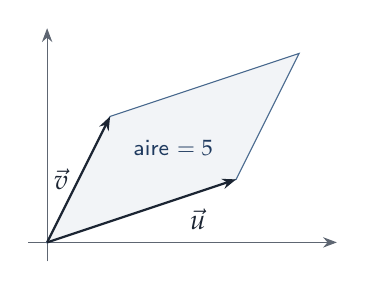
\begin{tikzpicture}[scale=0.8]
  \draw[->,Gris] (-0.3,0)--(4.6,0); \draw[->,Gris] (0,-0.3)--(0,3.4);
  \fill[Fond,draw=BleuMoyen] (0,0)--(3,1)--(4,3)--(1,2)--cycle;
  \draw[->,thick,Ink] (0,0)--(3,1) node[pos=0.7,below right]{$\ve u$};
  \draw[->,thick,Ink] (0,0)--(1,2) node[midway,left]{$\ve v$};
  \node[font=\footnotesize\sffamily,Bleu] at (2,1.5) {aire $=5$};
\end{tikzpicture}\\[4pt]
\only<3->{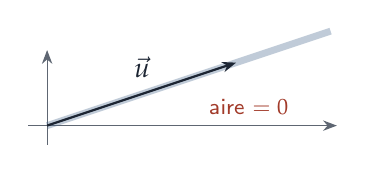
\begin{tikzpicture}[scale=0.8]
  \draw[->,Gris] (-0.3,0)--(4.6,0); \draw[->,Gris] (0,-0.3)--(0,1.2);
  \draw[BleuMoyen,line width=2.5pt,opacity=0.35] (0,0)--(4.5,1.5);
  \draw[->,thick,Ink] (0,0)--(3,1) node[pos=0.6,above left]{$\ve u$};
  \node[font=\footnotesize\sffamily,Brique] at (3.2,0.3) {aire $=0$};
\end{tikzpicture}}
\end{columns}
\end{frame}

\begin{frame}{Déterminant de deux vecteurs : une aire orientée}
\begin{columns}[c]
\column{0.55\textwidth}
\begin{FORM}[Déterminant 2×2 --- aire orientée]
$\ve u=(a,c)$, $\ve v=(b,d)$ dans une base orthonormée directe :
\[\det(\ve u,\ve v)=\dt{a&b\\c&d}=ad-bc\]\[\phantom{\det(\ve u,\ve v)}=\|\ve u\|\|\ve v\|\sin(\ve u,\ve v).\]
\end{FORM}
\pause
\begin{itemize}
\item \textbf{Valeur absolue} : aire du parallélogramme.
\item \textbf{Signe} : $+$ si l'on tourne de $\ve u$ vers $\ve v$ dans le sens direct.
\item $\det(\ve u,\ve v)=0\iff\ve u,\ve v$ colinéaires.
\end{itemize}
\column{0.4\textwidth}
\centering\onslide<1->
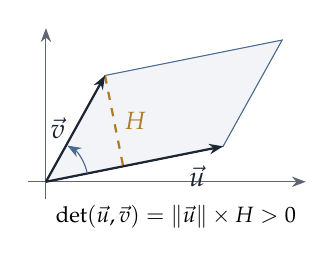
\begin{tikzpicture}[scale=0.75]
  \draw[->,Gris] (-0.3,0)--(4.4,0); \draw[->,Gris] (0,-0.3)--(0,2.6);
  \fill[Fond,draw=BleuMoyen] (0,0)--(3,0.6)--(4,2.4)--(1,1.8)--cycle;
  \draw[Ocre,dashed,thick] (1,1.8)--(1.3077,0.2615) node[midway,right,font=\small]{$H$};
  \draw[->,thick,Ink] (0,0)--(3,0.6) node[pos=0.75,below right]{$\ve u$};
  \draw[->,thick,Ink] (0,0)--(1,1.8) node[midway,left]{$\ve v$};
  \draw[->,BleuMoyen] (0.7,0.14) arc (11:60:0.7);
  \node[font=\footnotesize\sffamily] at (2.2,-0.6) {$\det(\ve u,\ve v)=\|\ve u\|\times H>0$};
\end{tikzpicture}\\[6pt]
\uncover<2->{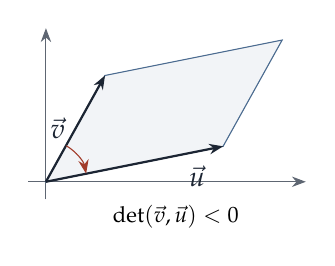
\begin{tikzpicture}[scale=0.75]
  \draw[->,Gris] (-0.3,0)--(4.4,0); \draw[->,Gris] (0,-0.3)--(0,2.6);
  \fill[Fond,draw=BleuMoyen] (0,0)--(3,0.6)--(4,2.4)--(1,1.8)--cycle;
  \draw[->,thick,Ink] (0,0)--(1,1.8) node[midway,left]{$\ve v$};
  \draw[->,thick,Ink] (0,0)--(3,0.6) node[pos=0.75,below right]{$\ve u$};
  \draw[->,Brique] (0.7*0.4903,0.7*0.8716) arc (60:11:0.7);
  \node[font=\footnotesize\sffamily] at (2.2,-0.6) {$\det(\ve v,\ve u)<0$};
\end{tikzpicture}}
\end{columns}
\end{frame}

\begin{frame}{Premier usage : inverser une matrice $2\times2$}
\begin{PROP}
Si $ad-bc\neq0$ :
\[\begin{pmatrix}a&b\\c&d\end{pmatrix}^{-1}=\dfrac1{ad-bc}\begin{pmatrix}d&-b\\-c&a\end{pmatrix}.\]
\end{PROP}
Mode d'emploi : \textbf{échanger la diagonale}, \textbf{changer les signes du reste}, \textbf{diviser par le déterminant}.
\pause
\begin{ATOI}
Inverser $A=\begin{pmatrix}3&1\\1&2\end{pmatrix}$, puis vérifier.
\end{ATOI}
\pause
\[\det A=6-1=5,\quad A^{-1}=\frac15\begin{pmatrix}2&-1\\-1&3\end{pmatrix},\quad
AA^{-1}=\frac15\begin{pmatrix}6-1&-3+3\\2-2&-1+6\end{pmatrix}=I_2.\ \ \rep{\checkmark}\]
\end{frame}

\begin{frame}{Dimension 3 : un volume orienté}
\begin{columns}[T]
\column{0.56\textwidth}
\begin{FORM}[Déterminant 3×3 --- volume orienté]
Colonnes $\ve u=(a,b,c)$, $\ve v=(d,e,f)$, $\ve w=(g,h,i)$ :
\[\dt{a&d&g\\b&e&h\\c&f&i}=a\dt{e&h\\f&i}-b\dt{d&g\\f&i}+c\dt{d&g\\e&h}.\]
\end{FORM}
\pause
\begin{itemize}
\item Produit mixte : $\det(\ve u,\ve v,\ve w)=(\ve u\wedge\ve v)\cdot\ve w$.
\item Volume $=|\det|$ = aire de base $\|\ve u\wedge\ve v\|$ $\times$ hauteur.
\item $\det=0\iff$ \textbf{coplanaires}.
\end{itemize}
\column{0.4\textwidth}
\centering\onslide<1->
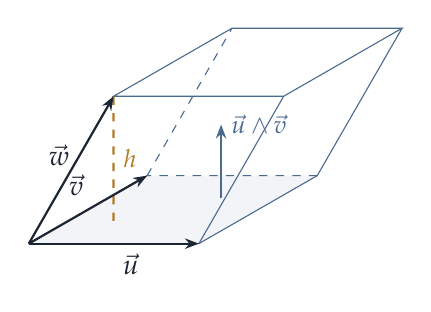
\begin{tikzpicture}[scale=0.72,x={(1cm,0cm)},y={(0.62cm,0.5cm)},z={(0cm,1cm)}]
  \coordinate (O) at (0,0,0); \coordinate (U) at (3,0,0); \coordinate (V) at (0.6,2.4,0); \coordinate (W) at (1,0.8,2.2);
  \coordinate (UV) at (3.6,2.4,0); \coordinate (UW) at (4,0.8,2.2); \coordinate (VW) at (1.6,3.2,2.2); \coordinate (UVW) at (4.6,3.2,2.2);
  \fill[Fond] (O)--(U)--(UV)--(V)--cycle;
  \draw[BleuMoyen] (O)--(U)--(UV); \draw[BleuMoyen,dashed] (UV)--(V)--(O);
  \draw[BleuMoyen] (U)--(UW) (UV)--(UVW); \draw[BleuMoyen,dashed] (V)--(VW);
  \draw[BleuMoyen] (W)--(UW)--(UVW)--(VW)--cycle;
  \draw[Ocre,dashed,thick] (1,0.8,0)--(W); \node[Ocre,font=\small,right] at (1,0.8,1.1) {$h$};
  \draw[->,thick,BleuMoyen] (2.4,1.6,0)--(2.4,1.6,1.3) node[right,font=\small]{$\ve u\wedge\ve v$};
  \draw[->,thick,Ink] (O)--(U) node[pos=0.6,below]{$\ve u$};
  \draw[->,thick,Ink] (O)--(V) node[pos=0.55,above left]{$\ve v$};
  \draw[->,thick,Ink] (O)--(W) node[pos=0.6,left]{$\ve w$};
\end{tikzpicture}
\end{columns}
\end{frame}

\begin{frame}{Calculer un $3\times3$ : à toi}
\begin{ATOI}
Calculer $D=\dt{1&0&2\\2&1&0\\0&3&1}$ de deux façons : développement selon la 1\textsuperscript{re} colonne, puis Sarrus.
\end{ATOI}
\pause
\textbf{Développement} (signes $+,-,+$) :
\[D=1\dt{1&0\\3&1}-2\dt{0&2\\3&1}+0=1\times1-2\times(0-6)=13.\]
\pause
\textbf{Sarrus} : $aei+dhc+gbf-ceg-fha-ibd=1+0+12-0-0-0=13$.\ \rep{\checkmark}
\pause
\begin{PIEGE}
Sarrus n'existe \emph{qu'en taille 3} ; au-delà : opérations et développement (§1.2).
\end{PIEGE}
\end{frame}

% =====================================================================
\partie{1.2}{Définition et règles de calcul}{En dimension $n$ on ne dessine plus : que garder de l'aire et du volume pour définir $\det$ ?}{\rmI}

\begin{frame}{Trois propriétés de l'aire orientée}
\begin{columns}[c]
\column{0.32\textwidth}\centering
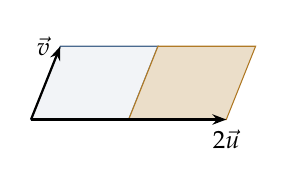
\begin{tikzpicture}[scale=0.62]
  \fill[Fond,draw=BleuMoyen] (0,0)--(2,0)--(2.6,1.5)--(0.6,1.5)--cycle;
  \fill[Ocre!25,draw=Ocre] (2,0)--(4,0)--(4.6,1.5)--(2.6,1.5)--cycle;
  \draw[->,thick] (0,0)--(4,0) node[below,font=\small]{$2\ve u$};
  \draw[->,thick] (0,0)--(0.6,1.5) node[left,font=\small]{$\ve v$};
\end{tikzpicture}\\[4pt]
\textbf{(i)} doubler un côté\\double l'aire
\column{0.32\textwidth}\centering
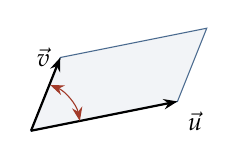
\begin{tikzpicture}[scale=0.62]
  \fill[Fond,draw=BleuMoyen] (0,0)--(3,0.6)--(3.6,2.1)--(0.6,1.5)--cycle;
  \draw[->,thick] (0,0)--(3,0.6) node[below right,font=\small]{$\ve u$};
  \draw[->,thick] (0,0)--(0.6,1.5) node[left,font=\small]{$\ve v$};
  \draw[<->,Brique] (1,0.2) arc (11:68:1);
\end{tikzpicture}\\[4pt]
\textbf{(ii)} échanger $\ve u,\ve v$\\inverse l'orientation
\column{0.32\textwidth}\centering
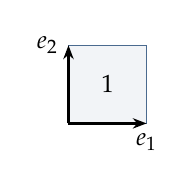
\begin{tikzpicture}[scale=0.62]
  \fill[Fond,draw=BleuMoyen] (0,0) rectangle (1.6,1.6);
  \draw[->,thick] (0,0)--(1.6,0) node[below,font=\small]{$e_1$};
  \draw[->,thick] (0,0)--(0,1.6) node[left,font=\small]{$e_2$};
  \node[font=\small] at (0.8,0.8) {$1$};
\end{tikzpicture}\\[4pt]
\textbf{(iii)} le carré unité\\a pour aire $1$
\end{columns}
\pause
\vspace{0.4cm}
\begin{center}
Ces trois propriétés \textbf{suffisent} à caractériser le déterminant, en toute dimension :\\
c'est la définition officielle.
\end{center}
\end{frame}

\begin{frame}{La définition}
\begin{DEF}[Définition --- théorème]
$\det:\Mn{\K}\to\K$ est l'\textbf{unique} application
\begin{enumerate}
\item[(i)] \textbf{linéaire par rapport à chaque colonne} (les autres fixées) :
      $\det(\dots,\lambda C_j+\mu C'_j,\dots)=\lambda\det(\dots,C_j,\dots)+\mu\det(\dots,C'_j,\dots)$ ;
\item[(ii)] \textbf{antisymétrique} : échanger deux colonnes change le signe ;
\item[(iii)] \textbf{normalisée} : $\det I_n=1$.
\end{enumerate}
\end{DEF}
\pause
\textbf{Lecture pratique :}
\begin{itemize}
\item (i) : on peut \alert{sortir un facteur} d'une colonne, et \alert{découper} une colonne en somme ;
\item (ii) : l'orientation ; \quad (iii) : le cube unité a pour volume $1$.
\end{itemize}
\end{frame}

\begin{frame}{La définition redonne la formule $ad-bc$}
Écrivons les colonnes dans la base $(e_1,e_2)$ : \quad $\det\big(ae_1+ce_2,\ be_1+de_2\big)$
\pause
\[\overset{\text{(i)}}{=}\ ab\det(e_1,e_1)+ad\det(e_1,e_2)+cb\det(e_2,e_1)+cd\det(e_2,e_2)\]
\pause
\begin{itemize}
\item (ii) : $\det(e_1,e_1)=-\det(e_1,e_1)$, donc $\det(e_1,e_1)=0$, de même $\det(e_2,e_2)=0$ ;
\item (ii) puis (iii) : $\det(e_2,e_1)=-\det(e_1,e_2)=-1$.
\end{itemize}
\pause
\[\det\big(ae_1+ce_2,\ be_1+de_2\big)=ad-bc.\qquad\rep{\text{On retrouve le §1.1.}}\]
\pause
\begin{RETENIR}
Toutes les règles de calcul qui suivent se démontrent \emph{uniquement} à partir de (i), (ii), (iii).
\end{RETENIR}
\end{frame}

\begin{frame}{Conséquences immédiates}
\begin{PROP}[Règles de calcul]
\renewcommand{\arraystretch}{1.25}
\begin{tabular}{@{}lll@{}}
$C_i\leftrightarrow C_j$ & (échange) & $\det\times(-1)$\\
$C_i\leftarrow\lambda C_i$ & (dilatation) & $\det\times\lambda$\\
$C_i\leftarrow C_i+\lambda C_j$, $j\neq i$ & (transvection) & $\det$ \textbf{inchangé}
\end{tabular}\\[3pt]
Colonne nulle, deux colonnes égales ou proportionnelles : $\det=0$.\qquad $\det(\lambda A)=\lambda^n\det A$.
\end{PROP}
\pause
\textbf{Pourquoi ?}
\begin{itemize}
\item Deux colonnes égales : les échanger ne change pas $A$ mais change le signe, donc $\det A=-\det A=0$.
\item Transvection, par (i) : $\det(\dots,C_i+\lambda C_j,\dots)=\det A+\lambda\underbrace{\det(\dots,C_j,\dots,C_j,\dots)}_{=0}$.
\item $\det(\lambda A)$ : on sort $\lambda$ de \emph{chacune} des $n$ colonnes.
\end{itemize}
\end{frame}

\begin{frame}{Développer selon une ligne ou une colonne}
\begin{PROP}[Théorème --- développement]
Pour toute ligne $i$ ou toute colonne $j$ :
\[\det A=\sum_j(-1)^{i+j}a_{i,j}\Delta_{i,j}=\sum_i(-1)^{i+j}a_{i,j}\Delta_{i,j},\]
$\Delta_{i,j}$ (\textbf{mineur}) : on supprime la ligne $i$ et la colonne $j$.
\end{PROP}
\begin{columns}[c]
\column{0.32\textwidth}\centering
Signes en damier :\\[3pt]
$\begin{pmatrix}+&-&+&\cdots\\-&+&-&\\+&-&+&\\\vdots&&&\ddots\end{pmatrix}$
\column{0.64\textwidth}
\pause
\begin{itemize}
\item On choisit la ligne ou colonne \alert{qui a le plus de zéros}.
\item Lignes et colonnes jouent le même rôle : $\det A^T=\det A$.
\item Le développement donne aussi une définition \emph{par récurrence} à partir de $ad-bc$.
\end{itemize}
\end{columns}
\end{frame}

\begin{frame}{Le cas idéal : une matrice triangulaire}
\begin{PROP}[Théorème]
Le déterminant d'une matrice triangulaire est le \textbf{produit de ses coefficients diagonaux}.
\end{PROP}
\pause
\textbf{Preuve} (récurrence) : la dernière ligne de $T$ est $(0,\dots,0,t_{n,n})$ ; on développe selon elle :
\[\det T=(-1)^{n+n}t_{n,n}\Delta_{n,n},\qquad\Delta_{n,n}\text{ triangulaire de diagonale }t_{1,1},\dots,t_{n-1,n-1}.\]
\pause
\begin{RETENIR}
Toute la stratégie de calcul en découle : \textbf{faire apparaître des zéros} par des transvections (qui ne changent pas $\det$),
jusqu'à une forme triangulaire ou une ligne à un seul coefficient.
\end{RETENIR}
\end{frame}

\begin{frame}{Méthode générale}
\begin{METH}{Calculer un déterminant}
\begin{enumerate}
\item \textbf{Regarder d'abord} la structure (tableau du §1.5) : colonnes liées ? somme constante ? ligne presque nulle ?
\item Sinon \textbf{pivot} : transvections pour créer des zéros (pivot $=1$ si possible), en notant échanges et facteurs
      sortis, jusqu'à une forme triangulaire ou une ligne/colonne à un seul coefficient ; développer selon elle.
\item Avec paramètre : \textbf{sortir les facteurs} dès qu'ils apparaissent ; ne jamais tout développer.
\end{enumerate}
\end{METH}
\end{frame}

\begin{frame}{Les pièges du calcul}
\begin{PIEGE}[Pièges]
\begin{itemize}
\item $\det(A+B)\neq\det A+\det B$ ;\quad $\det(\lambda A)\neq\lambda\det A$.
\item Transvection : la colonne modifiée garde le coefficient $1$ ($C_i\leftarrow2C_i+C_j$ multiplie par $2$).
\item Opérations successives : chacune agit sur la matrice \emph{déjà} modifiée.
\item Oublier le signe $(-1)^{i+j}$ du développement.
\end{itemize}
\end{PIEGE}
\end{frame}

\begin{frame}{Exemple : regarder avant de calculer}
\begin{columns}[c]
\column{0.4\textwidth}
\[D=\dt{1&2&3&4\\4&1&2&3\\3&4&1&2\\2&3&4&1}\]
\column{0.56\textwidth}
\begin{ATOI}
Avant tout calcul : que remarques-tu sur les lignes ?
\end{ATOI}
\end{columns}
\pause
\rep{Chaque ligne a pour somme $10$.} \ D'où : $C_1\leftarrow C_1+C_2+C_3+C_4$, puis on sort $10$ :
\pause
\[D=10\dt{1&2&3&4\\1&1&2&3\\1&4&1&2\\1&3&4&1}\overset{L_i-L_1}{=}10\dt{1&2&3&4\\0&-1&-1&-1\\0&2&-2&-2\\0&1&1&-3}
=10\dt{-1&-1&-1\\2&-2&-2\\1&1&-3}\]
\pause
$C_2-C_1$, $C_3-C_1$ : \ $\dt{-1&0&0\\2&-4&-4\\1&0&-4}=-1\times16=-16$, \ donc \ $\boxed{D=-160}$.
\end{frame}

% ---------------------------------------------------------------- EXERCICE D1
\begin{frame}{\badgeexo{1}Les règles de calcul en action}
\begin{ENONCE}[5 min]
\begin{enumerate}
\item Calculer $\dt{1&2&1\\2&5&3\\-1&1&4}$ par opérations sur les lignes.
\item Sans aucun calcul : que vaut $\dt{1&2&3\\4&5&6\\7&8&9}$ ?
\item $A\in\mathcal M_3(\R)$ avec $\det A=5$. Que vaut $\det(2A)$ ? et $\det(-A^T)$ ?
\end{enumerate}
\objectif{transvections, colonnes liées, $\det(\lambda A)=\lambda^n\det A$. Indice pour 2 : comparer $C_1+C_3$ et $C_2$.}
\end{ENONCE}
\end{frame}

\begin{frame}{\badgecor{1}Les règles de calcul en action}
\begin{columns}[T]
\column{0.38\textwidth}
\begin{RAIS}
Créer des zéros par transvections (déterminant inchangé), repérer une relation entre colonnes, compter les facteurs sortis.
\end{RAIS}
\begin{OUTIL}
Règles de calcul (§1.2) ; colonnes liées $\Rightarrow\det=0$.
\end{OUTIL}
\column{0.59\textwidth}
\etape{1.} $L_2\leftarrow L_2-2L_1$, $L_3\leftarrow L_3+L_1$ :
$\dt{1&2&1\\0&1&1\\0&3&5}=1\times(5-3)=2$.\\[3pt]
\pause
\etape{2.} $C_1+C_3=2C_2$ : colonnes liées, le déterminant est \textbf{nul}.\\[3pt]
\pause
\etape{3.} $\det(2A)=2^3\cdot5=40$ ; \ $\det(-A^T)=(-1)^3\det A=-5$.
\end{columns}
{\small\color{Brique}\textbf{Piège :} $\det(2A)\neq2\det A$, les trois colonnes sont multipliées par $2$.}
\end{frame}

% =====================================================================
\partie{1.3}{Propriétés globales, endomorphismes}{Que dit le déterminant d'une matrice, d'un produit, d'un endomorphisme ?}{\rmI}

\begin{frame}{Le théorème fondamental}
\begin{PROP}[Théorème fondamental]
$A$ inversible $\iff\det A\neq0\iff$ colonnes libres.\\[3pt]
$\det(AB)=\det A\det B$ ;\quad $\det A^{-1}=\dfrac1{\det A}$ ;\quad $\det A^T=\det A$ ;\quad $\det(PBP^{-1})=\det B$.
\end{PROP}
\pause
\textbf{Idée de preuve.}
\begin{itemize}
\item Colonnes liées : $C_i=\sum_{j\neq i}\lambda_jC_j$ ; la transvection $C_i\leftarrow C_i-\sum\lambda_jC_j$ crée une colonne nulle : $\det A=0$.
\item $A$ inversible : $\det A\det A^{-1}=\det I_n=1$, donc $\det A\neq0$.
\end{itemize}
\pause
\begin{PIEGE}
Le déterminant est \emph{multiplicatif}, pas additif : il passe aux produits, inverses, transposées, jamais aux sommes.
\end{PIEGE}
\end{frame}

\begin{frame}{Des questions sans aucun coefficient}
\begin{METH}{Question sans coefficients}
Une relation entre matrices $\Rightarrow$ on applique $\det$ aux deux membres.
\end{METH}
\begin{ATOI}
$A\in\Mn{\R}$ vérifie $A^2=-I_n$. Que peut-on dire de $n$ ?
\end{ATOI}
\pause
$(\det A)^2=\det(-I_n)=(-1)^n$. Un carré réel est $\geq0$, donc \rep{$n$ est pair}.\quad
\alert{Faux dans $\C$} : $A=iI_n$.
\pause
\begin{ATOI}
$A$ antisymétrique ($A^T=-A$) d'ordre $n$ impair : $\det A$ ?
\end{ATOI}
\pause
$\det A=\det A^T=\det(-A)=(-1)^n\det A=-\det A$, donc \rep{$\det A=0$}.
\pause\par
\textbf{Autre cas :} $A^2=A$, $A\neq I_n$ : $\det A\in\{0,1\}$, et $\det A=1$ forcerait $A=I_n$ ; donc $\det A=0$.
\end{frame}

\begin{frame}{Déterminant d'une famille, d'un endomorphisme}
\begin{DEF}
$\det_{\mathcal B}(u_1,\dots,u_n)$ : déterminant des coordonnées des $u_j$ dans la base $\mathcal B$.\\
$\det f=\det\Mat_{\mathcal B}(f)$ \ --- \ indépendant de $\mathcal B$ (matrices semblables).
\end{DEF}
\begin{PROP}
$(u_1,\dots,u_n)$ base de $E$ ($\dim E=n$) $\iff\det_{\mathcal B}(u_j)\neq0$ ;\quad $f$ automorphisme $\iff\det f\neq0$.\\
$\det(f\circ g)=\det f\det g$,\quad $\det(\lambda f)=\lambda^n\det f$,\quad $\det f^{-1}=\frac1{\det f}$.
\end{PROP}
\pause
\begin{EX}
$(1,\,1+X,\,\dots,\,1+X+\dots+X^n)$ : base de $\R_n[X]$ (triangulaire, diagonale de $1$).\\
Dérivation $D$ sur $\R_n[X]$ : diagonale nulle, $\det D=0$ : non bijective.
\end{EX}
\end{frame}

\begin{frame}{Le bon réflexe : la base adaptée}
\begin{columns}[c]
\column{0.58\textwidth}
\begin{PROP}[Projecteurs, symétries]
Projecteur $p$ : $\det p=1$ si $p=\Id$, $0$ sinon.\\[2pt]
Symétrie $s$ :\ \ $\det s=(-1)^{\dim\mathrm{Ker}(s+\Id)}=(-1)^{n-\rg(s+\Id)}$.
\end{PROP}
\pause
\textbf{Pourquoi :} dans une base adaptée,
\[\Mat p=\mathrm{diag}(I_r,0),\qquad\Mat s=\mathrm{diag}(I_r,-I_{n-r}).\]
\pause
\begin{RETENIR}
Endomorphisme défini géométriquement $\Rightarrow$ \textbf{base adaptée}, jamais la base canonique.
\end{RETENIR}
\column{0.38\textwidth}\centering\onslide<1->
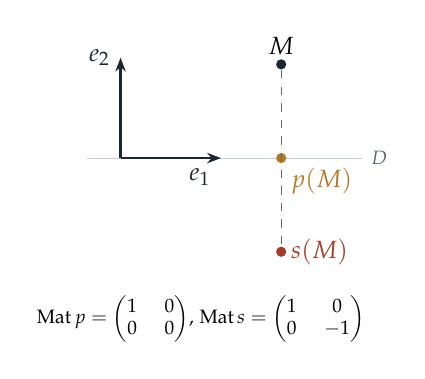
\begin{tikzpicture}[scale=0.85]
  \draw[Filet] (-0.5,0)--(3.6,0) node[right,font=\scriptsize,Gris]{$D$};
  \draw[->,thick,Ink] (0,0)--(1.5,0) node[below left,font=\small]{$e_1$};
  \draw[->,thick,Ink] (0,0)--(0,1.5) node[left,font=\small]{$e_2$};
  \node[pt] (M) at (2.4,1.4) {}; \node[font=\small,above] at (M) {$M$};
  \node[pt,fill=Ocre] (P) at (2.4,0) {}; \node[font=\small,below right,Ocre] at (P) {$p(M)$};
  \node[pt,fill=Brique] (S) at (2.4,-1.4) {}; \node[font=\small,right,Brique] at (S) {$s(M)$};
  \draw[dashed,Gris] (M)--(S);
  \node[font=\scriptsize,align=left] at (1.2,-2.4) {$\Mat p=\begin{pmatrix}1&0\\0&0\end{pmatrix}$,\ $\Mat s=\begin{pmatrix}1&0\\0&-1\end{pmatrix}$};
\end{tikzpicture}\\
{\scriptsize projection sur $D$ et réflexion d'axe $D$ :\\ $\det p=0$, $\det s=-1$}
\end{columns}
\end{frame}

\begin{frame}{Base adaptée : deux exemples de TD}
\begin{EX}[$f:M\mapsto AM$ sur $\mathcal M_2(\R)$]
Base $(E_{11},E_{21},E_{12},E_{22})$ : on agit colonne par colonne, donc $\Mat f=\mathrm{diag}(A,A)$ et
$\det f=(\det A)^2$ \ (en taille $n$ : $(\det A)^n$).
\end{EX}
\pause
\begin{FORM}[Similitudes \HP{} --- TD 8]
$\C$ vu comme $\R$-espace vectoriel, base $(1,i)$, $a=\alpha+i\beta$ :
\begin{itemize}
\item $z\mapsto az$ : $\begin{pmatrix}\alpha&-\beta\\\beta&\alpha\end{pmatrix}$, $\det=|a|^2$, $\mathrm{tr}=2\,\mathrm{Re}\,a$ ;
      symétrie $\iff a=\pm1$ ; $|a|=1$ : rotation d'angle $\arg a$.
\item $z\mapsto a\bar z$ : $\begin{pmatrix}\alpha&\beta\\\beta&-\alpha\end{pmatrix}$, $\det=-|a|^2$ ; réflexion si $|a|=1$.
\end{itemize}
$\det f>0$ : orientation conservée ; $<0$ : renversée.
\end{FORM}
\end{frame}

% ---------------------------------------------------------------- EXERCICE D2
\begin{frame}{\badgeexo{2}Déterminant d'un endomorphisme}
\begin{ENONCE}[6 min]
Calculer le déterminant des endomorphismes suivants, en choisissant une base adaptée.
\begin{enumerate}
\item $T:\mathcal M_2(\R)\to\mathcal M_2(\R)$, $M\mapsto M^T$.
\item $g:\R_2[X]\to\R_2[X]$, $P\mapsto P(X+1)$. Est-ce un automorphisme ?
\end{enumerate}
\objectif{ne jamais calculer dans une base mal choisie.}
\end{ENONCE}
\pause
\begin{INDICE}
1 : matrices symétriques, matrices antisymétriques. \quad 2 : images de $1$, $X$, $X^2$.
\end{INDICE}
\end{frame}

\begin{frame}{\badgecor{2}Déterminant d'un endomorphisme}
\begin{columns}[T]
\column{0.38\textwidth}
\begin{RAIS}
$\det f$ ne dépend pas de la base : on prend celle où la matrice est diagonale ou triangulaire.
\end{RAIS}
\begin{OUTIL}
$\det f=\det\Mat_{\mathcal B}(f)$ ; matrice triangulaire.
\end{OUTIL}
\column{0.59\textwidth}
\etape{1.} Base $\big(E_{11},E_{22},E_{12}+E_{21}\big)$ (symétriques, $T=\Id$) complétée par $E_{12}-E_{21}$ (antisymétrique, $T=-\Id$) :
$\Mat(T)=\mathrm{diag}(1,1,1,-1)$, \ $\det T=-1$.\\[3pt]
\pause
\etape{2.} $g(1)=1$, $g(X)=1+X$, $g(X^2)=1+2X+X^2$ : dans $(1,X,X^2)$,
$\Mat(g)=\begin{pmatrix}1&1&1\\0&1&2\\0&0&1\end{pmatrix}$, triangulaire : $\det g=1\neq0$, \textbf{automorphisme}.
\end{columns}
\end{frame}

\begin{frame}{Pour aller plus loin : la comatrice \HP}
\begin{HPBOX}
$\com(A)=\big((-1)^{i+j}\Delta_{i,j}\big)$ \ (matrice des cofacteurs). Pour toute $A$ :
\[A\,\com(A)^T=\com(A)^TA=\det(A)\,I_n,\]
donc, si $\det A\neq0$ :\quad $A^{-1}=\dfrac1{\det A}\com(A)^T$.
\end{HPBOX}
\pause
\textbf{Pourquoi :} le coefficient $(i,i)$ de $A\,\com(A)^T$ est le développement de $\det A$ selon la ligne $i$ ; le
coefficient $(k,i)$, $k\neq i$, développe une matrice à deux lignes égales : $0$.
\pause
\begin{itemize}
\item En taille 2 : la formule du §1.1 ;\quad $\det\com(A)=(\det A)^{n-1}$.
\item $A$ entière : $A^{-1}$ entière $\iff\det A=\pm1$.
\end{itemize}
\begin{PIEGE}
\emph{Transposer} la comatrice ; mettre le signe $(-1)^{i+j}$ sur chaque cofacteur.
\end{PIEGE}
\end{frame}

% =====================================================================
\partie{1.4}{Géométrie}{Comment traduire « alignés », « coplanaires », « aire », « distance » par un déterminant ?}{\rmI}

\begin{frame}{Le dictionnaire géométrique}
\begin{FORM}[Traductions (base orthonormée)]
\renewcommand{\arraystretch}{1.35}
\begin{tabular}{@{}ll@{}}
$A,B,C$ alignés & $\det(\vv{AB},\vv{AC})=0$\\
$M(x,y)\in(BC)$ & $\dt{1&1&1\\x&b&c\\y&b'&c'}=0$\\
$M\in(ABC)$ & $\det(\vv{AM},\vv{AB},\vv{AC})=0$\\
aire du triangle $ABC$ & $\frac12|\det(\vv{AB},\vv{AC})|$\\
volume du tétraèdre $ABCD$ & $\frac16|\det(\vv{AB},\vv{AC},\vv{AD})|$\\
$A+\vect\ve u$, $C+\vect\ve v$ coplanaires & $\det(\vv{AC},\ve u,\ve v)=0$
\end{tabular}\\[2pt]
{\small Pour $(BC)$, avec $B(b,b')$, $C(c,c')$ : $C_1-C_2$, $C_3-C_2$ donnent $-\det(\vv{BM},\vv{BC})$.}
\end{FORM}
\end{frame}

\begin{frame}{Le dictionnaire en action}
\begin{ATOI}
$A(1,2)$, $B(2,-2)$, $C(3,1)$ : aire du triangle ? Équation de $(AB)$ ?
\end{ATOI}
\pause
\begin{itemize}
\item $\vv{AB}=(1,-4)$, $\vv{AC}=(2,-1)$ :\quad $\det(\vv{AB},\vv{AC})=\dt{1&2\\-4&-1}=7$ :\quad \rep{aire $\frac72$}.
\pause
\item $M(x,y)\in(AB)\iff\dt{1&x-1\\-4&y-2}=0\iff$ \rep{$y=-4x+6$}.
\end{itemize}
\pause
\begin{ASTU}
On écrit toujours la condition sous la forme « $\det=0$ » : l'équation sort directement, sans calculer de pente.
\end{ASTU}
\end{frame}

\begin{frame}{Distance de deux droites de l'espace}
\begin{columns}[c]
\column{0.5\textwidth}
\begin{FORM}[Distance --- TD 2]
$\mathcal D_1=A+\vect\ve u$, $\mathcal D_2=C+\vect\ve v$ non parallèles :
\[d(\mathcal D_1,\mathcal D_2)=\frac{|\det(\vv{AC},\ve u,\ve v)|}{\|\ve u\wedge\ve v\|}.\]
\end{FORM}
\pause
\textbf{Lecture :} $|\det(\vv{AC},\ve u,\ve v)|$ est le volume du parallélépipède de base $\|\ve u\wedge\ve v\|$ et de
hauteur $d$ : \alert{volume / base}.
\pause\par\smallskip
\textbf{Perpendiculaire commune :} $H=A+s\ve u$, $K=C+r\ve v$ avec $\vv{HK}\cdot\ve u=\vv{HK}\cdot\ve v=0$.\\
Sécantes $\iff d=0$.
\column{0.47\textwidth}\centering\onslide<1->
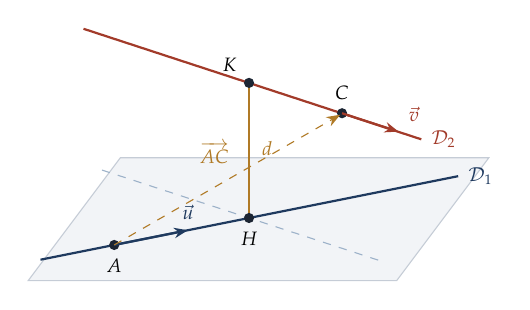
\begin{tikzpicture}[scale=0.78]
\fill[Fond] (0,0)--(6,0)--(7.5,2)--(1.5,2)--cycle; \draw[Filet] (0,0)--(6,0)--(7.5,2)--(1.5,2)--cycle;
\draw[Bleu,thick] (0.2,0.34)--(7.0,1.70) node[right,font=\scriptsize]{$\mathcal D_1$};
\draw[BleuClair,dashed] (1.2,1.8)--(5.8,0.3);
\draw[Brique,thick] (0.9,4.1)--(6.4,2.3) node[right,font=\scriptsize]{$\mathcal D_2$};
\draw[Ocre,thick] (3.595,1.019)--(3.595,3.219);
\node[pt] at (3.595,1.019) {}; \node[font=\scriptsize,anchor=north] at (3.595,0.95) {$H$};
\node[pt] at (3.595,3.219) {}; \node[font=\scriptsize,anchor=south east] at (3.55,3.25) {$K$};
\node[font=\scriptsize,Ocre,anchor=west] at (3.65,2.15) {$d$};
\node[pt] at (1.4,0.58) {}; \node[font=\scriptsize,anchor=north] at (1.4,0.52) {$A$};
\draw[->,Bleu,thick] (1.4,0.58)--(2.6,0.82) node[above,font=\scriptsize]{$\ve u$};
\node[pt] at (5.11,2.725) {}; \node[font=\scriptsize,anchor=south] at (5.11,2.78) {$C$};
\draw[->,Brique,thick] (5.11,2.725)--(6.03,2.425) node[above right,font=\scriptsize]{$\ve v$};
\draw[->,Ocre,dashed] (1.4,0.58)--(5.08,2.70) node[pos=0.55,above left,font=\scriptsize]{$\vv{AC}$};
\end{tikzpicture}\\
{\scriptsize Plan gris : contient $\mathcal D_1$, parallèle à $\mathcal D_2$.}
\end{columns}
\end{frame}

% ---------------------------------------------------------------- EXERCICE D3
\begin{frame}{\badgeexo{3}Coplanaires ? Quel volume ?}
\begin{ENONCE}[5 min]
Dans l'espace muni d'un repère orthonormé, $A(1,2,0)$, $B(2,3,1)$, $C(0,1,1)$, $D(1,1,2)$.
\begin{enumerate}
\item Les quatre points sont-ils coplanaires ?
\item Calculer le volume du tétraèdre $ABCD$.
\end{enumerate}
\objectif{le dictionnaire géométrique du §1.4.}
\end{ENONCE}
\end{frame}

\begin{frame}{\badgecor{3}Coplanaires ? Quel volume ?}
\begin{columns}[T]
\column{0.38\textwidth}
\begin{RAIS}
Coplanaires $\iff\det(\vv{AB},\vv{AC},\vv{AD})=0$ ; sinon, ce déterminant est le volume orienté du parallélépipède, le tétraèdre
en vaut le sixième.
\end{RAIS}
\column{0.59\textwidth}
\etape{1.} $\vv{AB}=(1,1,1)$, $\vv{AC}=(-1,-1,1)$, $\vv{AD}=(0,-1,2)$. Avec $C_2\leftarrow C_2+C_1$ :
\[\dt{1&-1&0\\1&-1&-1\\1&1&2}=\dt{1&0&0\\1&0&-1\\1&2&2}=2.\]
Non nul : \textbf{non coplanaires}.\\[3pt]
\pause
\etape{2.} $\mathcal V=\frac16|2|=\frac13$.
\end{columns}
\end{frame}

% =====================================================================
\partie{1.5}{Quelle méthode pour quel déterminant ?}{Face à un déterminant d'ordre $n$, comment choisir la bonne technique avant de calculer ?}{\rmI}

\begin{frame}{La carte des méthodes}
\footnotesize
\renewcommand{\arraystretch}{1.12}
\begin{tabular}{@{}>{\raggedright}p{0.42\linewidth}>{\raggedright\arraybackslash}p{0.48\linewidth}r@{}}
\toprule
\textsf{\footnotesize Je vois\dots} & \textsf{\footnotesize Je fais\dots} & \\\midrule
colonnes combinaisons de $\leq2$ vecteurs ($i+j$\dots) & $\det=0$ ($n\geq3$) & \\
même somme sur chaque ligne & $C_1\leftarrow\sum C_j$, sortir la somme, $L_i-L_1$ & \textcolor{Ocre}{1.6}\\
$a_{i,j}$ formule ($\max$, $|i-j|$, $a^{|i-j|}$) & $C_k-C_{k-1}$ (ou $-aC_{k-1}$), $k=n\to2$ & \textcolor{Ocre}{1.6}\\
ligne/colonne à 1 coefficient & développer selon elle & \textcolor{Ocre}{1.2}\\
lettres X, Z, N & développer ; permuter lignes \emph{et} colonnes & \textcolor{Ocre}{1.6}\\
puissances $1,x,x^2,\dots$ & Vandermonde / polynôme en $x$ & \textcolor{Ocre}{1.6}\\
tridiagonal & récurrence d'ordre 2 & \textcolor{Ocre}{1.6}\\
$a$ au-dessus, $b$ au-dessous, constante ajoutée & fonction affine ; $a=b$ par dérivée & \textcolor{Ocre}{1.6}\\
relation entre matrices & $\det(AB)$, $\det(\lambda A)$, $\det A^T$ & \textcolor{Ocre}{1.3}\\
endomorphisme géométrique & base adaptée & \textcolor{Ocre}{1.3}\\
\bottomrule
\end{tabular}\\[4pt]
{\footnotesize\color{Gris}Ce tableau est le §1.5 de la fiche : on y revient au début de chaque exercice.}
\end{frame}

% =====================================================================
\partie{1.6}{Techniques d'ordre $n$}{Comment calculer un déterminant dont la taille $n$ est une lettre ?}{\rmI}

\begin{frame}{Somme constante}
\begin{columns}[c]
\column{0.36\textwidth}
\[D_n(a,b)=\dt{a&b&\cdots&b\\b&a&\ddots&\vdots\\\vdots&\ddots&\ddots&b\\b&\cdots&b&a}\]
\column{0.6\textwidth}
\pause
\begin{enumerate}
\item Chaque ligne a pour somme $a+(n-1)b$ : $C_1\leftarrow C_1+\dots+C_n$, on sort ce facteur.
\item $L_i\leftarrow L_i-L_1$ ($i\geq2$) : triangulaire de diagonale $(1,a-b,\dots,a-b)$.
\end{enumerate}
\end{columns}
\pause
\begin{FORM}
\[D_n(a,b)=\big(a+(n-1)b\big)(a-b)^{n-1}.\]
Inversible $\iff a\neq b$ et $a+(n-1)b\neq0$ \ ($n\geq2$). \quad C'est la matrice $(a-b)I_n+bJ$ du TD 6.
\end{FORM}
\end{frame}

\begin{frame}{Formule en $i,j$ : les différences successives}
\begin{METH}{Différences successives}
$C_k\leftarrow C_k-C_{k-1}$ pour $k=n,n-1,\dots,2$ (\textbf{depuis la fin} : chaque opération utilise une colonne intacte).
Nouveau coefficient : distinguer $i<k$ et $i\geq k$.
\end{METH}
\pause
\textbf{Exemple} $a_{i,j}=\max(i,j)$, $n=4$ :
\[\begin{pmatrix}1&2&3&4\\2&2&3&4\\3&3&3&4\\4&4&4&4\end{pmatrix}\ \longrightarrow\
\begin{pmatrix}1&1&1&1\\2&0&1&1\\3&0&0&1\\4&0&0&0\end{pmatrix}\]
\pause
Dernière ligne $(n,0,\dots,0)$ : on développe, le mineur est triangulaire à diagonale de $1$ :
\[\det\big(\max(i,j)\big)=(-1)^{n+1}n\qquad(\text{ici }-4).\]
\end{frame}

\begin{frame}{Différences successives : résultats à connaître}
\begin{FORM}[Résultats]
\renewcommand{\arraystretch}{1.3}
\begin{tabular}{@{}ll@{}}
$\det\big(\max(i,j)\big)=(-1)^{n+1}n$ & dernière ligne $(n,0,\dots,0)$\\
$\det\big(|i-j|\big)=(-1)^{n-1}(n-1)2^{n-2}$ & colonnes, puis $L_i-L_{i-1}$, puis $C_1+\frac12\sum_{k\geq2}C_k$\\
$\det\big(a^{|i-j|}\big)=(1-a^2)^{n-1}$ & avec $C_k-aC_{k-1}$
\end{tabular}
\end{FORM}
\pause
\begin{ATOI}[Contrôle]
Vérifier la formule $|i-j|$ pour $n=2$, $n=3$.
\end{ATOI}
\pause
\[n=2:\ \dt{0&1\\1&0}=-1=(-1)^1\cdot1\cdot2^0\ \rep{\checkmark}\quad
n=3:\ \dt{0&1&2\\1&0&1\\2&1&0}=4=(-1)^2\cdot2\cdot2\ \rep{\checkmark}\]
\end{frame}

% ---------------------------------------------------------------- EXERCICE D4
\begin{frame}{\badgeexo{4}La matrice $\min(i,j)$}
\begin{ENONCE}[5 min]
Pour $n\geq1$, calculer $\Delta_n=\det\big(\min(i,j)\big)_{1\leq i,j\leq n}$, par exemple
$\Delta_4=\dt{1&1&1&1\\1&2&2&2\\1&2&3&3\\1&2&3&4}$.
\objectif{les différences successives, dans le bon ordre.}
\end{ENONCE}
\pause
\begin{INDICE}
Que vaut la ligne $L_i-L_{i-1}$ ? Par quelle ligne commencer ?
\end{INDICE}
\end{frame}

\begin{frame}{\badgecor{4}La matrice $\min(i,j)$}
\begin{columns}[T]
\column{0.38\textwidth}
\begin{RAIS}
Deux lignes consécutives ne diffèrent que sur la fin : leurs différences font apparaître une matrice triangulaire.
\end{RAIS}
\begin{OUTIL}
Différences successives (§1.6) ; matrice triangulaire.
\end{OUTIL}
\column{0.59\textwidth}
\etape{1.} $L_i-L_{i-1}=(0,\dots,0,1,\dots,1)$, le premier $1$ en colonne $i$.\\[3pt]
\etape{2.} On fait $L_n\leftarrow L_n-L_{n-1}$, puis $L_{n-1}\leftarrow L_{n-1}-L_{n-2}$, \dots, $L_2\leftarrow L_2-L_1$ :
\emph{chaque opération utilise une ligne pas encore modifiée}.\\[3pt]
\pause
\etape{3.} La matrice obtenue est triangulaire supérieure, de diagonale $(1,\dots,1)$ : $\Delta_n=1$.
\end{columns}
\begin{PIEGE}
Commencer par $L_2-L_1$ puis $L_3-L_2$ utiliserait une ligne \emph{déjà modifiée}.
\end{PIEGE}
\end{frame}

\begin{frame}{Déterminants creux : X, Z, N}
\begin{columns}[c]
\column{0.3\textwidth}\centering
$\begin{pmatrix}a&&&b\\&a&b&\\&b&a&\\b&&&a\end{pmatrix}$\\[2pt]{\scriptsize « X » d'ordre $4$}
\column{0.66\textwidth}
\begin{ASTU}[Astuces]
\begin{itemize}
\item Permuter lignes et colonnes par la \emph{même} permutation ne change pas $\det$ ($P^{-1}AP$) : on regroupe en blocs.
\item Inverser l'ordre de $m$ lignes : $\lfloor m/2\rfloor$ échanges.
\item Ligne à un seul coefficient : la sortir, puis s'en servir de pivot.
\end{itemize}
\end{ASTU}
\end{columns}
\pause
\textbf{X d'ordre $2n$ :} réordonner selon $1,2n,2,2n-1,\dots$ : $n$ blocs $\begin{pmatrix}a&b\\b&a\end{pmatrix}$, d'où
$(a^2-b^2)^n$.
\end{frame}

\begin{frame}{Déterminants creux : résultats}
\begin{FORM}[Résultats --- TD 4, TD 9]
X d'ordre $2n$ : $(a^2-b^2)^n$ ; ordre $2n+1$ (centre $a$) : $a(a^2-b^2)^n$.\\
Z d'ordre $n$ : $(-1)^{\lfloor\frac{n-2}2\rfloor}b_2\cdots b_{n-1}(a_1c_n-a_nc_1)$ ;\quad
N ($b_j$ sur la diagonale) : $b_2\cdots b_{n-1}(a_1c_n-a_nc_1)$.
\end{FORM}
\pause
\begin{PIEGE}
Le signe de l'anti-diagonale : le $b$ de la première ligne est en position $(1,2n)$, de signe $(-1)^{2n+1}=-1$.
Une erreur de signe donnerait $(a^2+b^2)^n$, faux dès $n=1$.
\end{PIEGE}
\pause
\begin{RETENIR}
Toujours tester la formule finale sur $n=3$ ou $4$.
\end{RETENIR}
\end{frame}

\begin{frame}{Vandermonde}
\begin{FORM}[Théorème --- Vandermonde]
\[V(x_1,\dots,x_n)=\det\big(x_j^{\,i-1}\big)=\dt{1&1&\cdots&1\\x_1&x_2&\cdots&x_n\\\vdots&&&\vdots\\x_1^{n-1}&x_2^{n-1}&\cdots&x_n^{n-1}}=\prod_{i<j}(x_j-x_i),\]
non nul $\iff$ les $x_i$ sont distincts.\quad $n=3$ : $(b-a)(c-a)(c-b)$.
\end{FORM}
\pause
\textbf{D'où vient le produit ?} Regardons la dernière variable comme une inconnue $x$ : c'est la méthode suivante.
\end{frame}

\begin{frame}{Voir un déterminant comme un polynôme}
\begin{METH}{Polynôme en $x$}
$x$ dans une seule colonne $\Rightarrow$ développer selon elle : $P(x)$ est un polynôme.
\begin{enumerate}
\item Coefficient dominant = cofacteur de la plus haute puissance.
\item Racines évidentes : valeurs rendant deux colonnes égales.
\item Autant de racines que le degré $\Rightarrow P=$ coeff.\ dominant $\times\prod(x-\text{racine})$.
\end{enumerate}
\end{METH}
\pause
\textbf{Exemple :} $P(x)=\dt{1&1&1\\a&b&x\\a^2&b^2&x^2}$ ($a\neq b$).
\pause
\begin{itemize}
\item Degré $\leq2$, coefficient de $x^2$ : $\dt{1&1\\a&b}=b-a$ ;\quad $P(a)=P(b)=0$ (colonnes égales).
\end{itemize}
\pause
\[P(x)=(b-a)(x-a)(x-b)\qquad\Rightarrow\qquad V(a,b,c)=(b-a)(c-a)(c-b).\]
\end{frame}

\begin{frame}{Polynôme en $x$ : deux précautions}
\begin{PIEGE}[Piège : un terme manquant]
Une puissance manque (pas de $x^2$) : une racine de plus à trouver.
\[\dt{1&1&1\\a&b&c\\a^3&b^3&c^3}=(b-a)(c-a)(c-b)(a+b+c).\]
\end{PIEGE}
\pause
\begin{PIEGE}[Piège : racines non distinctes]
Racines supposées distinctes ; en cas d'égalité, \textbf{les deux membres sont nuls} : le dire.
\end{PIEGE}
\pause
\begin{RETENIR}
Coefficient dominant + racines évidentes + degré : trois informations suffisent, sans développer.
\end{RETENIR}
\end{frame}

\begin{frame}{Tridiagonal : une récurrence}
\begin{columns}[c]
\column{0.38\textwidth}
\[T_n=\dt{a&b&&\\c&a&\ddots&\\&\ddots&\ddots&b\\&&c&a}\]
\column{0.58\textwidth}
\pause
\begin{enumerate}
\item Développer selon $L_1$ : $T_n=aT_{n-1}-b\,(\cdots)$.
\item Le 2\textsuperscript{e} mineur commence par la colonne $(c,0,\dots,0)$ : le développer selon $C_1$.
\end{enumerate}
\end{columns}
\pause
\begin{METH}{Récurrence}
\[T_n=aT_{n-1}-bc\,T_{n-2}\qquad(\text{seul le produit }bc\text{ compte}).\]
Poser $T_0=1$ (compatible) ; \textbf{vérifier $T_3$ à la main}.
\end{METH}
\end{frame}

\begin{frame}{Résoudre la récurrence : exemple du TD 3}
\begin{FORM}[Suites récurrentes linéaires d'ordre 2]
$u_n=\alpha u_{n-1}+\beta u_{n-2}$, équation $r^2=\alpha r+\beta$ :\quad
racines distinctes : $\lambda r_1^n+\mu r_2^n$ ;\quad racine double : $(\lambda+\mu n)r^n$ ;\quad
$\rho e^{\pm i\theta}$ : $\rho^n(\lambda\cos n\theta+\mu\sin n\theta)$.
\end{FORM}
\pause
\textbf{Diagonale $5$, $6$ au-dessus, $1$ au-dessous :}\quad $T_n=5T_{n-1}-6T_{n-2}$.
\pause
\begin{itemize}
\item $r^2=5r-6$ : $r_1=2$, $r_2=3$, donc $T_n=\lambda2^n+\mu3^n$.
\item $T_0=1$, $T_1=5$ : $\lambda+\mu=1$, $2\lambda+3\mu=5$, d'où $\mu=3$, $\lambda=-2$.
\end{itemize}
\pause
\[\boxed{T_n=3^{n+1}-2^{n+1}}\qquad T_2=19,\ T_3=65,\ T_4=211.\]
\end{frame}

\begin{frame}{Tridiagonaux à connaître}
\begin{FORM}[À connaître]
Diagonale $2\cos\theta$, $1$ de part et d'autre : $\dfrac{\sin(n+1)\theta}{\sin\theta}$ (TD 7) ; diagonale $2$, $-1$ de part et
d'autre : $n+1$.\\
Outil : $\sin(n+1)\theta+\sin(n-1)\theta=2\sin n\theta\cos\theta$.
\end{FORM}
\pause
\begin{ATOI}[Contrôle]
Vérifier $\frac{\sin(n+1)\theta}{\sin\theta}$ pour $n=1$ et $n=2$.
\end{ATOI}
\pause
$n=1$ : $\frac{\sin2\theta}{\sin\theta}=2\cos\theta=T_1$ \rep{\checkmark}.\qquad
$n=2$ : $T_2=4\cos^2\theta-1$ et $\frac{\sin3\theta}{\sin\theta}=4\cos^2\theta-1$ \rep{\checkmark}.
\end{frame}

\begin{frame}{Une constante ajoutée partout : fonction affine}
\begin{METH}{Fonction affine}
$D(x)$ = déterminant avec $x$ ajouté (ou retranché) à tous les coefficients : $C_j-C_1$ chassent $x$ sauf de $C_1$,
donc $D$ est \textbf{affine}. On choisit les $x$ qui rendent la matrice triangulaire.
\end{METH}
\pause
\begin{FORM}[$\lambda_i$ sur la diagonale, $a$ au-dessus, $b$ au-dessous --- TD 10]
$Q(x)=\prod(\lambda_i-x)$, $P(x)=\det(A_n-xU)$ ($U$ : que des $1$) : \ $P(a)=Q(a)$, $P(b)=Q(b)$, et $\det A_n=P(0)$ :
\[\det A_n=\frac{b\,Q(a)-a\,Q(b)}{b-a}\quad(a\neq b),\qquad\det A_n=Q(a)-aQ'(a)\quad(a=b).\]
\end{FORM}
\pause
{\small $a=b$ : continuité, puis taux d'accroissement de $\varphi(u)=uQ(a)-aQ(u)$ ($\varphi(a)=0$).\
Exemple : diagonale $x$, $1$ au-dessus, $-1$ au-dessous : $\frac{(x+1)^n+(x-1)^n}2$.}
\end{frame}

\begin{frame}{Chapitre 1 : ce qu'il faut retenir}
\begin{RETENIR}
\begin{enumerate}
\item $\det$ = volume orienté ; \textbf{nul $\iff$ vecteurs liés $\iff$ non inversible}.
\item Définition : linéaire par colonne, antisymétrique, $\det I_n=1$ ; d'où les règles de calcul.
\item Transvections $\Rightarrow$ zéros $\Rightarrow$ développement ou triangulaire.
\item Multiplicatif : $\det(AB)$, $\det A^{-1}$, $\det A^T$, $\det(\lambda A)=\lambda^n\det A$ --- jamais $\det(A+B)$.
\item Endomorphisme : \textbf{base adaptée}. Géométrie : alignement, aire, volume, distance.
\item Ordre $n$ : \textbf{regarder la structure} d'abord (carte du §1.5).
\end{enumerate}
\end{RETENIR}
\pause
\textbf{Au travail :} TD 1 à 10 de déterminants, avec la fiche (§1.1 à §1.7 : résultats des TD pour se corriger).
\end{frame}

% =====================================================================
%                CHAPITRE 2 — COURBES PARAMÉTRÉES PLANES
% =====================================================================
\chapitre{Chapitre 2 · Courbes paramétrées planes}
\def\fichesec{}
\newcommand{\rmII}{\rmitem{2.1}{Fonctions vectorielles, outils de calcul}\rmitem{2.2}{Tangente, pente}\rmitem{2.3}{Plan d'étude, symétries, tracé}
  \rmitem{2.4}{Points stationnaires, étude locale, inflexions}\rmitem{2.5}{Branches infinies, positions}\rmitem{2.6}{Intersections, points doubles}
  \rmitem{2.7}{Check-list et résultats des TD}}

\begin{frame}[plain]
\begin{tikzpicture}[remember picture,overlay]
  \fill[Bleu] (current page.north west) rectangle (current page.south east);
  \fill[Ocre] ([yshift=-4.2cm]current page.north west) rectangle ([yshift=-4.25cm,xshift=5cm]current page.north west);
  \node[anchor=north west,text=white!70!Bleu,font=\sffamily\small] at ([xshift=1cm,yshift=-1.6cm]current page.north west) {Chapitre 2};
  \node[anchor=north west,text=white,font=\sffamily\bfseries\fontsize{28}{30}\selectfont] at ([xshift=1cm,yshift=-2.3cm]current page.north west) {Courbes paramétrées};
  \node[anchor=north west,text width=8.5cm,text=white,font=\large] at ([xshift=1cm,yshift=-4.7cm]current page.north west)
    {Décrire une courbe par un point mobile $M(t)$.\\[2pt]
     \normalsize\color{white!75!Bleu} Étudier une courbe, c'est savoir la tracer avec ses points remarquables, ses tangentes et ses
     branches infinies.};
  \begin{axis}[at={([xshift=-5.3cm,yshift=-7.6cm]current page.north east)},anchor=south west,width=4.6cm,height=6.6cm,hide axis,
     xmin=-1.3,xmax=1.3,ymin=-2.3,ymax=2.3,samples=300,smooth]
   \addplot[white,line width=1.4pt,domain=0:6.2832]({cos(3*x)},{2*sin(x)});
  \end{axis}
\end{tikzpicture}
\end{frame}

% =====================================================================
\partie{2.1}{Fonctions vectorielles, outils de calcul}{Pourquoi décrire une courbe par $t\mapsto M(t)$ plutôt que par $y=g(x)$ ?}{\rmII}

\begin{frame}{Quand $y=g(x)$ ne suffit plus}
\begin{columns}[c]
\column{0.55\textwidth}
Un cercle, une boucle : à une abscisse correspondent \alert{plusieurs points}. On décrit alors la courbe par un \textbf{point
mobile}.
\pause
\begin{DEF}
Courbe paramétrée : $f:I\to\R^2$ (ou $\R^3$) de classe $\mathcal C^1$,
\[f(t)=\vv{OM(t)}=\big(x(t),y(t)\big).\]
Support : $\{M(t),\ t\in I\}$.
\end{DEF}
\pause
Équation cartésienne $F(x,y)=0$ $\neq$ représentation paramétrique.
\column{0.4\textwidth}\centering\onslide<1->
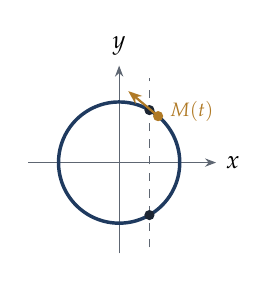
\begin{tikzpicture}
\begin{axis}[courbe,width=4.6cm,xmin=-1.5,xmax=1.6,ymin=-1.5,ymax=1.6,xtick=\empty,ytick=\empty]
\addplot[arcetude,domain=0:6.2832]({cos(x)},{sin(x)});
\draw[Gris,dashed] (axis cs:0.5,-1.4)--(axis cs:0.5,1.4);
\node[pt] at (axis cs:0.5,0.866) {}; \node[pt] at (axis cs:0.5,-0.866) {};
\node[pt,fill=Ocre] at (axis cs:0.643,0.766) {};
\draw[->,Ocre,thick] (axis cs:0.643,0.766)--(axis cs:0.15,1.18);
\node[font=\scriptsize,Ocre,anchor=west] at (axis cs:0.68,0.85) {$M(t)$};
\end{axis}
\end{tikzpicture}\\
{\scriptsize deux points pour la même abscisse ;\\ le point $M(t)$ et sa vitesse}
\end{columns}
\end{frame}

\begin{frame}{Trois paramétrages à savoir écrire}
\begin{EX}[Exemples du livre]
\begin{itemize}
\item \textbf{Droite} par $A(1,2)$ et $B(2,-2)$ : $t\mapsto A+t\vv{AB}$ ; équation $y=-4x+6$.
\item \textbf{Cercle} de centre $\Omega$, rayon $R$ : $\theta\mapsto\Omega+R(\cos\theta,\sin\theta)$, $\theta\in\,]-\pi,\pi]$.
\item \textbf{Graphe} $y=g(x)$ : $t\mapsto\big(t,g(t)\big)$.
\end{itemize}
\end{EX}
\pause
\begin{ATOI}
Paramétrer le cercle $(x-1)^2+(y-2)^2=R^2$. Quelle partie est le graphe de $x\mapsto2+\sqrt{R^2-(x-1)^2}$ ?
\end{ATOI}
\pause
\rep{$\theta\mapsto(1+R\cos\theta,\ 2+R\sin\theta)$} ; le graphe est le \rep{demi-cercle $y\geq2$}.
\end{frame}

\begin{frame}{Dériver une fonction vectorielle}
\begin{FORM}[Dérivation]
Tout se lit \textbf{sur les coordonnées} : $f'=(x',y')$ vitesse, $f''$ accélération, $\|f'\|$ vitesse scalaire.
\[(\lambda f+g)'=\lambda f'+g',\quad(\varphi f)'=\varphi'f+\varphi f',\quad(f\circ\varphi)'=\varphi'\,(f'\circ\varphi),\]
\[(f\cdot g)'=f'\cdot g+f\cdot g',\quad(f\wedge g)'=f'\wedge g+f\wedge g'\ (\R^3),\]
\[\text{Leibniz : }(\varphi f)^{(n)}=\textstyle\sum_{k=0}^n\binom nk\varphi^{(k)}f^{(n-k)}.\]
Taylor--Young : $f(t_0+h)=\sum_{k=0}^n\frac{h^k}{k!}f^{(k)}(t_0)+o(h^n)$.
\end{FORM}
\pause
\textbf{Exemple type :} $\|f\|$ constante $\Rightarrow$ on dérive $f\cdot f$ : $f\cdot f'=0$ (mouvement circulaire : vitesse $\perp$ rayon).
\end{frame}

\begin{frame}{La boîte à outils de calcul}
\begin{columns}[T]
\column{0.47\textwidth}
\begin{FORM}[DL en 0]
$\frac1{1+u}=1-u+u^2-u^3+o(u^3)$\\[2pt]
$\ln(1+u)=u-\frac{u^2}2+\frac{u^3}3+o(u^3)$\\[2pt]
$e^u=1+u+\frac{u^2}2+\frac{u^3}6+o(u^3)$\\[2pt]
$\sqrt{1+u}=1+\frac u2-\frac{u^2}8+\frac{u^3}{16}+o(u^3)$
\end{FORM}
\begin{METH}{En $t_0\neq0$ ou à l'infini}
$t=t_0+h$ ; faire apparaître $1+u$.\\
Inverse : $e^t-1=t(1+u)$, puis $\frac1{1+u}$.\\
À l'infini : factoriser le terme dominant.
\end{METH}
\column{0.49\textwidth}
\begin{FORM}[Trigonométrie]
$1-\cos t=2\sin^2\frac t2$,\ \ $\sin t=2\sin\frac t2\cos\frac t2$\\[2pt]
$\cos3t=4\cos^3t-3\cos t$\\[2pt]
$\sin3t=\sin t\,(4\cos^2t-1)$\\[2pt]
Angle moitié :\\
$e^{ia}\pm e^{ib}=e^{i\frac{a+b}2}\big(e^{i\frac{a-b}2}\pm e^{-i\frac{a-b}2}\big)$\\[2pt]
$\cos t-\cos2t=2\sin\frac t2\sin\frac{3t}2$\\[2pt]
$\cos t+\cos2t=2\cos\frac t2\cos\frac{3t}2$
\end{FORM}
\end{columns}
{\footnotesize\color{Gris}Liste complète (linéarisations, $\sin$, $\cos$ à l'ordre 5) : fiche §2.1.}
\end{frame}

% =====================================================================
\partie{2.2}{Tangente, pente}{Comment trouver la tangente en un point, même quand la courbe n'est pas un graphe ?}{\rmII}

\begin{frame}{De la corde à la tangente}
\begin{columns}[c]
\column{0.52\textwidth}
\begin{DEF}
Tangente en $M(t_0)$ : position limite de la droite $M(t_0)+\vect(\ve u_h)$, où $\ve u_h$ est le vecteur \textbf{unitaire}
dirigeant la corde $[M(t_0)M(t_0+h)]$.
\end{DEF}
\pause
Pourquoi normaliser ? $\vv{M(t_0)M(t_0+h)}\to\ve0$ ne donne, seul, aucune direction.
\pause
\begin{DEF}
$M(t_0)$ \textbf{régulier} si $f'(t_0)\neq\ve0$, \textbf{stationnaire} sinon. Courbe régulière : tous ses points réguliers.
\end{DEF}
\column{0.44\textwidth}\centering\onslide<1->
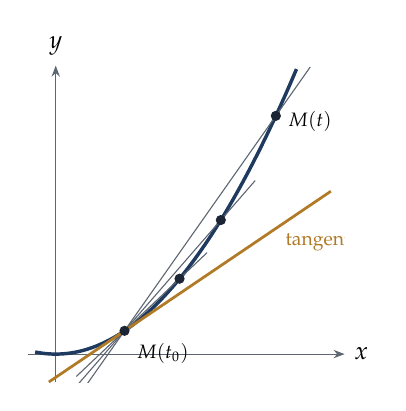
\begin{tikzpicture}
\begin{axis}[courbe,width=5.6cm,height=5.6cm,xmin=-0.2,xmax=2.1,ymin=-0.3,ymax=3.1,xtick=\empty,ytick=\empty,axis equal image=false]
\addplot[arcetude,domain=-0.15:1.75]({x},{x^2});
\addplot[Gris,thin,domain=0.15:1.85,samples=2]{0.25+2.1*(x-0.5)};
\addplot[Gris,thin,domain=0.15:1.45,samples=2]{0.25+1.7*(x-0.5)};
\addplot[Gris,thin,domain=0.15:1.1,samples=2]{0.25+1.4*(x-0.5)};
\addplot[tgte,domain=-0.05:2.0,samples=2]{x-0.25};
\node[pt] at (axis cs:0.5,0.25) {}; \node[font=\scriptsize,anchor=north west] at (axis cs:0.52,0.22) {$M(t_0)$};
\node[pt] at (axis cs:1.6,2.56) {}; \node[pt] at (axis cs:1.2,1.44) {}; \node[pt] at (axis cs:0.9,0.81) {};
\node[font=\scriptsize,anchor=west] at (axis cs:1.62,2.5) {$M(t)$};
\node[font=\scriptsize,Ocre,anchor=west] at (axis cs:1.6,1.2) {tangente};
\end{axis}
\end{tikzpicture}\\
{\scriptsize les cordes pivotent vers la tangente}
\end{columns}
\end{frame}

\begin{frame}{Tangente en un point régulier}
\begin{PROP}[Théorème]
En un point régulier : $T=M(t_0)+\vect f'(t_0)$, d'équation
\[\det\big(\vv{M(t_0)M},f'(t_0)\big)=0\iff y'_0(x-x_0)-x'_0(y-y_0)=0.\]
Horizontale $\iff y'(t_0)=0$ ;\quad verticale $\iff x'(t_0)=0$ \ (point régulier !).
\end{PROP}
\pause
\textbf{Preuve :} Taylor--Young à l'ordre 1, $\vv{M(t_0)M(t_0+h)}=h\big(f'(t_0)+o(1)\big)$, donc
$\ve u_h\to\pm\frac{f'(t_0)}{\|f'(t_0)\|}$ : les deux limites dirigent la même droite.
\end{frame}

\begin{frame}{Exemple : tangente à une ellipse}
\begin{ATOI}
Ellipse $f(\theta)=(2\cos\theta,\sin\theta)$ : tangente en $\theta=\frac\pi4$ ?
\end{ATOI}
\pause
\begin{columns}[c]
\column{0.58\textwidth}
\begin{itemize}
\item $M_0=\big(\sqrt2,\frac{\sqrt2}2\big)$, \ $f'\big(\frac\pi4\big)=\big(-\sqrt2,\frac{\sqrt2}2\big)\neq\ve0$ : régulier.
\pause
\item $y'_0(x-x_0)-x'_0(y-y_0)=0$ :
\[\tfrac{\sqrt2}2(x-\sqrt2)+\sqrt2\big(y-\tfrac{\sqrt2}2\big)=0\]
\[\iff\ \rep{x+2y-2\sqrt2=0}.\]
\end{itemize}
\column{0.38\textwidth}\centering\onslide<1->
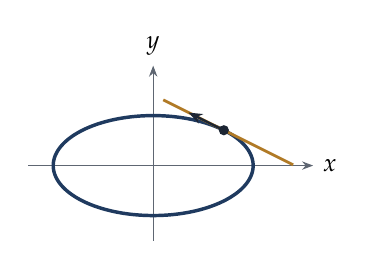
\begin{tikzpicture}
\begin{axis}[courbe,width=5.2cm,xmin=-2.5,xmax=3.2,ymin=-1.5,ymax=2,xtick=\empty,ytick=\empty]
\addplot[arcetude,domain=0:6.2832]({2*cos(x)},{sin(x)});
\uncover<3->{\addplot[tgte,samples=2,domain=0.2:2.8]{(2*sqrt(2)-x)/2};}
\node[pt] at (axis cs:1.414,0.707) {};
\uncover<2->{\draw[->,thick,Ink] (axis cs:1.414,0.707)--(axis cs:0.707,1.06);}
\end{axis}
\end{tikzpicture}
\end{columns}
\end{frame}

% ---------------------------------------------------------------- EXERCICE C1
\begin{frame}{\badgeexo{5}Tangentes horizontales, verticales, en un point}
\begin{ENONCE}[5 min]
Soit $f(t)=\big(t^2,\ t^3-3t\big)$, $t\in\R$.
\begin{enumerate}
\item Déterminer les points où la tangente est horizontale, puis verticale.
\item Donner une équation de la tangente au point de paramètre $t=2$.
\end{enumerate}
\objectif{tangente dirigée par $f'(t)$ en un point régulier.}
\end{ENONCE}
\end{frame}

\begin{frame}{\badgecor{5}Tangentes horizontales, verticales, en un point}
\begin{columns}[T]
\column{0.38\textwidth}
\begin{RAIS}
En un point régulier, la tangente est dirigée par $f'(t)=(x'(t),y'(t))$ : horizontale si $y'=0$, verticale si $x'=0$.
\end{RAIS}
\begin{OUTIL}
Tangente en un point régulier : $\det\big(M-f(t_0),\,f'(t_0)\big)=0$.
\end{OUTIL}
\column{0.59\textwidth}
\etape{1.} $f'(t)=(2t,\ 3t^2-3)$. Horizontale : $t=\pm1$ ($x'\neq0$), points $(1,-2)$ et $(1,2)$.
Verticale : $t=0$ ($y'(0)=-3\neq0$), point $(0,0)$.\\[3pt]
\pause
\etape{2.} $f(2)=(4,2)$, $f'(2)=(4,9)$ :
\[\dt{x-4&4\\y-2&9}=0\iff9x-4y-28=0.\]
\end{columns}
\end{frame}

\begin{frame}{D'où vient la pente $\dfrac{y'}{x'}$ ?}
Si $x'(t_0)\neq0$, $x$ est strictement monotone près de $t_0$ : localement, la courbe est un \textbf{graphe}
\[y(t)=g\big(x(t)\big).\]
\pause
On dérive la composée :\qquad $y'(t)=g'\big(x(t)\big)\,x'(t)$,\qquad donc\qquad
\[\boxed{\ \text{pente}=g'\big(x(t_0)\big)=\frac{y'(t_0)}{x'(t_0)}\ }\]
\pause
\begin{columns}[T]
\column{0.48\textwidth}
\begin{FORM}[Usages]
Parallèle à $\ve w$ : $\det(f',\ve w)=0$.\\
Pente $m$ : $y'=m\,x'$.
\end{FORM}
\column{0.48\textwidth}
\begin{PIEGE}[Pièges]
« $x'=0$ donc verticale » : faux si $y'=0$ aussi.\\
$\frac yx$ = pente de $(OM)$, pas de la tangente.
\end{PIEGE}
\end{columns}
\end{frame}

% =====================================================================
\partie{2.3}{Plan d'étude, symétries, tracé}{Dans quel ordre étudier une courbe pour la tracer sans rien oublier ?}{\rmII}

\begin{frame}{Le plan d'étude en 6 étapes}
\begin{center}
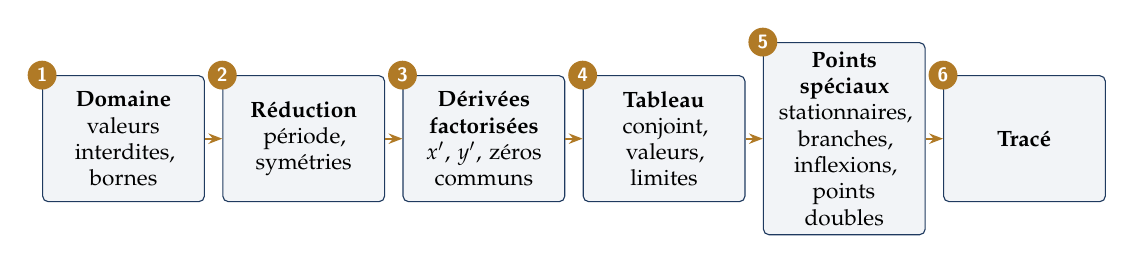
\begin{tikzpicture}[node distance=0.22cm,
  st/.style={rectangle,rounded corners=2pt,draw=Bleu,fill=Fond,text width=1.82cm,minimum height=1.6cm,align=center,font=\footnotesize},
  nb/.style={circle,fill=Ocre,text=white,font=\sffamily\bfseries\scriptsize,inner sep=1.5pt}]
\node[st] (a) {\textbf{Domaine}\\ valeurs interdites, bornes};
\node[st,right=of a] (b) {\textbf{Réduction}\\ période, symétries};
\node[st,right=of b] (c) {\textbf{Dérivées factorisées}\\ $x'$, $y'$, zéros communs};
\node[st,right=of c] (d) {\textbf{Tableau} conjoint, valeurs, limites};
\node[st,right=of d] (e) {\textbf{Points\\ spéciaux}\\ stationnaires, branches, inflexions, points doubles};
\node[st,right=of e] (f) {\textbf{Tracé}};
\foreach \n/\k in {a/1,b/2,c/3,d/4,e/5,f/6}{\node[nb] at (\n.north west) {\k};}
\foreach \x/\y in {a/b,b/c,c/d,d/e,e/f}{\draw[->,Ocre,thick] (\x)--(\y);}
\end{tikzpicture}
\end{center}
\pause
\begin{itemize}
\item Étape 3 : \alert{même dénominateur, facteurs affines} : les signes se lisent directement.
\item Étape 5 : stationnaires (§2.4), branches (§2.5), points doubles (§2.6).
\item Étape 6 : on complète par les symétries \textbf{dans l'ordre inverse} des réductions.
\end{itemize}
\end{frame}

\begin{frame}{Réduire le domaine : les symétries}
\begin{columns}[c]
\column{0.58\textwidth}
\textbf{Principe :} chercher $\varphi$ ($t\mapsto-t$, $\pi-t$, $\frac1t$\dots) telle que $M(\varphi(t))=s\big(M(t)\big)$.
\begin{FORM}[Table des symétries]
\small\renewcommand{\arraystretch}{1.1}
\begin{tabular}{@{}lll@{}}
$f(-t)=(x,-y)$ & axe $(Ox)$ & $t\geq0$\\
$f(-t)=(-x,y)$ & axe $(Oy)$ & $t\geq0$\\
$f(-t)=-f(t)$ & centre $O$ & $t\geq0$\\
$f(\frac1t)=(y,x)$ & axe $y=x$ & $|t|\leq1$\\
$f(\pi-t)=(\pm x,\pm y)$ & selon signes & demi-intervalle\\
$f(t+T)=f(t)$ & période & une période
\end{tabular}
\end{FORM}
\column{0.38\textwidth}\centering\onslide<1->
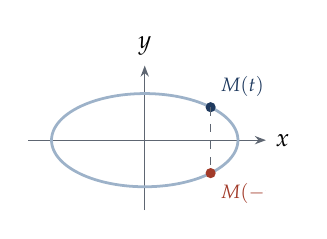
\begin{tikzpicture}
\begin{axis}[courbe,width=4.6cm,xmin=-2.5,xmax=2.6,ymin=-1.5,ymax=1.6,xtick=\empty,ytick=\empty]
\addplot[reste,domain=0:6.2832]({2*cos(x)},{sin(x)});
\node[pt,fill=Bleu] at (axis cs:1.414,0.707) {}; \node[font=\scriptsize,anchor=south west,Bleu] at (axis cs:1.42,0.72) {$M(t)$};
\node[pt,fill=Brique] at (axis cs:1.414,-0.707) {}; \node[font=\scriptsize,anchor=north west,Brique] at (axis cs:1.42,-0.72) {$M(-t)$};
\draw[Gris,dashed] (axis cs:1.414,0.707)--(axis cs:1.414,-0.707);
\end{axis}
\end{tikzpicture}\\
{\scriptsize $x$ paire, $y$ impaire : symétrie d'axe $(Ox)$}
\end{columns}
\end{frame}

% ---------------------------------------------------------------- EXERCICE C2
\begin{frame}{\badgeexo{6}Réduire l'intervalle d'étude}
\begin{ENONCE}[5 min]
Soit $f(t)=\big(\sin2t,\ \sin3t\big)$. Réduire l'intervalle d'étude au maximum, en précisant à chaque étape la transformation
géométrique qui permet de reconstituer la courbe.
\objectif{périodicité, puis $f(-t)$, puis $f(\pi-t)$.}
\end{ENONCE}
\end{frame}

\begin{frame}{\badgecor{6}Réduire l'intervalle d'étude}
\begin{columns}[T]
\column{0.38\textwidth}
\begin{RAIS}
On compare $f(t+T)$, $f(-t)$, $f(a-t)$ à $(\pm x,\pm y)$ : chaque relation divise l'intervalle par $2$ et fournit une symétrie.
\end{RAIS}
\begin{OUTIL}
Réduction par les symétries (§2.3).
\end{OUTIL}
\column{0.59\textwidth}
\etape{1.} $f$ est $2\pi$-périodique : étude sur $[-\pi,\pi]$.\\[3pt]
\etape{2.} $f(-t)=(-x,-y)$ : symétrie de centre $O$ ; étude sur $[0,\pi]$.\\[3pt]
\pause
\etape{3.} $f(\pi-t)=\big(\sin(2\pi-2t),\sin(3\pi-3t)\big)=(-x,\,y)$ : symétrie d'axe $(Oy)$ ; étude sur $\left[0,\frac\pi2\right]$.\\[3pt]
Reconstitution : arc sur $\left[0,\frac\pi2\right]$, symétrique par rapport à $(Oy)$, puis par rapport à $O$.
\end{columns}
\end{frame}

\begin{frame}{Exemple : l'ellipse $f(\theta)=(2\cos\theta,\sin\theta)$}
\begin{columns}[c]
\column{0.55\textwidth}
\begin{enumerate}
\item $2\pi$-périodique.\pause
\item $x$ paire, $y$ impaire : \textbf{axe $(Ox)$}, étude sur $[0,\pi]$.\pause
\item $f(\pi-\theta)=(-x,y)$ : \textbf{axe $(Oy)$}, étude sur $\big[0,\frac\pi2\big]$.\pause
\item Sur $\big[0,\frac\pi2\big]$ : $x\searrow$ de $2$ à $0$, $y\nearrow$ de $0$ à $1$ ; tangente verticale en $(2,0)$
      ($f'(0)=(0,1)$), horizontale en $(0,1)$.\pause
\item Compléter : axe $(Oy)$, puis axe $(Ox)$.
\end{enumerate}
\column{0.4\textwidth}\centering\onslide<1->
\begin{tikzpicture}
\begin{axis}[courbe,width=5.4cm,xmin=-2.5,xmax=2.6,ymin=-1.5,ymax=1.6,xtick={-2,2},ytick={-1,1}]
\only<5->{\addplot[reste,domain=1.5708:3.1416]({2*cos(x)},{sin(x)});}
\only<5->{\addplot[reste,domain=3.1416:6.2832]({2*cos(x)},{sin(x)});}
\only<4->{\addplot[arcetude,domain=0:1.5708]({2*cos(x)},{sin(x)});
\addplot[tgte,samples=2,domain=-0.4:0.4]({2},{x});\addplot[tgte,samples=2,domain=-0.6:0.6]({x},{1});}
\end{axis}
\end{tikzpicture}\\
{\scriptsize arc étudié (foncé), puis complété par symétries}
\end{columns}
\end{frame}

\begin{frame}{Du tableau au tracé}
\begin{columns}[c]
\column{0.4\textwidth}\centering\onslide<1->
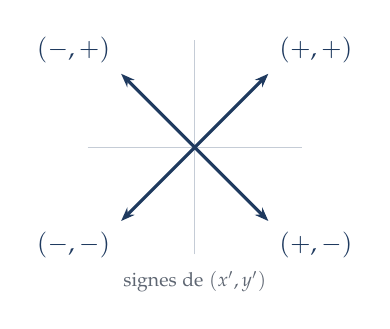
\begin{tikzpicture}[scale=0.85]
\draw[Filet] (-1.6,0)--(1.6,0) (0,-1.6)--(0,1.6);
\draw[->,Bleu,very thick] (0,0)--(1.1,1.1) node[above right,font=\small]{$(+,+)$};
\draw[->,Bleu,very thick] (0,0)--(1.1,-1.1) node[below right,font=\small]{$(+,-)$};
\draw[->,Bleu,very thick] (0,0)--(-1.1,1.1) node[above left,font=\small]{$(-,+)$};
\draw[->,Bleu,very thick] (0,0)--(-1.1,-1.1) node[below left,font=\small]{$(-,-)$};
\node[font=\scriptsize,Gris] at (0,-2) {signes de $(x',y')$};
\end{tikzpicture}
\column{0.56\textwidth}
\begin{METH}{Tracer}
\begin{enumerate}
\item Asymptotes en pointillés ; points nommés avec un segment de tangente.
\item Arcs selon le tableau : direction donnée par les signes de $(x',y')$.
\item Positions (asymptotes, tangentes) ; symétries ; flèches de sens.
\end{enumerate}
\end{METH}
\end{columns}
\pause
\begin{ASTU}[Astuces]
Point sur un axe de symétrie : tangente $\perp$ à l'axe, sauf point stationnaire ou double.
Symétrie supposée : vérifier la compatibilité ($f$ impaire $\Rightarrow f(0)=O$).
\end{ASTU}
\end{frame}

% =====================================================================
\partie{2.4}{Points stationnaires, étude locale, inflexions}{Que se passe-t-il quand la vitesse s'annule ? Quand la courbe traverse-t-elle sa tangente ?}{\rmII}

\begin{frame}{Les quatre allures locales}
\begin{center}
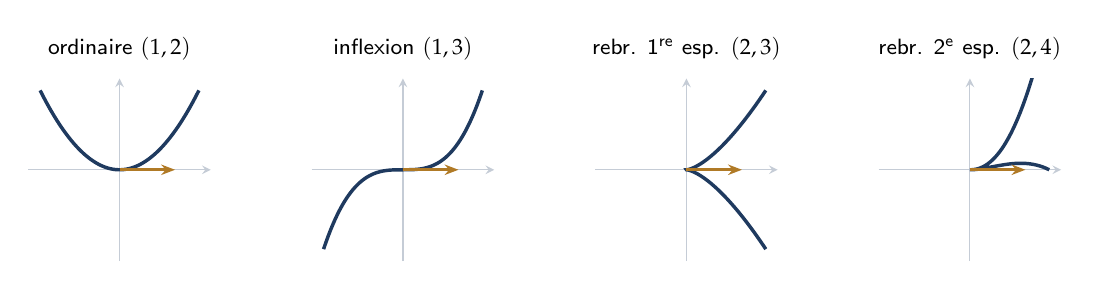
\begin{tikzpicture}
\begin{axis}[mini,title={ordinaire $(1,2)$}]\addplot[arcetude,domain=-1:1]({x},{x^2});\draw[tgte,->](axis cs:0,0)--(axis cs:0.7,0);\end{axis}
\begin{axis}[mini,xshift=3.6cm,title={inflexion $(1,3)$}]\addplot[arcetude,domain=-1:1]({x},{x^3});\draw[tgte,->](axis cs:0,0)--(axis cs:0.7,0);\end{axis}
\begin{axis}[mini,xshift=7.2cm,title={rebr. 1\textsuperscript{re} esp. $(2,3)$}]\addplot[arcetude,domain=-1:1]({x^2},{x^3});\draw[tgte,->](axis cs:0,0)--(axis cs:0.7,0);\end{axis}
\begin{axis}[mini,xshift=10.8cm,title={rebr. 2\textsuperscript{e} esp. $(2,4)$}]\addplot[arcetude,domain=-1:1]({x^2},{x^4+x^5});\draw[tgte,->](axis cs:0,0)--(axis cs:0.7,0);\end{axis}
\end{tikzpicture}
\end{center}
\pause
\begin{DEF}
\textbf{Ordinaire} : la courbe reste du même côté de sa tangente. \textbf{Inflexion} : elle la traverse.
\textbf{Rebroussement} : elle s'arrête et repart en arrière, en traversant sa tangente (1\textsuperscript{re} espèce) ou non
(2\textsuperscript{e}). \textbf{Anguleux} : demi-tangentes non colinéaires ($(t,|t|)$).
\end{DEF}
\pause
Modèle $(t^p,t^q)$ en $O$ : la corde $\frac{(t^p,t^q)}{t^p}=(1,t^{q-p})\to(1,0)$ ; les \textbf{parités} de $p,q$ décident.
\end{frame}

\begin{frame}{Le théorème $(p,q)$}
\begin{PROP}[Théorème $(p,q)$]
$p=\min\{k\geq1:f^{(k)}(t_0)\neq\ve0\}$, \ $q=\min\{k>p:(f^{(p)},f^{(k)})\text{ libre}\}$. Tangente dirigée par $f^{(p)}(t_0)$.
\begin{center}
\renewcommand{\arraystretch}{1.2}
\begin{tabular}{c|cc}
 & $q$ pair & $q$ impair\\\hline
$p$ impair & ordinaire & inflexion\\
$p$ pair & rebr. 2\textsuperscript{e} esp. & rebr. 1\textsuperscript{re} esp.
\end{tabular}
\end{center}
\end{PROP}
\pause
\textbf{Pourquoi :} dans le repère $\big(M_0,f^{(p)}(t_0),f^{(q)}(t_0)\big)$, \ $X\sim\frac{h^p}{p!}$, $Y\sim\frac{h^q}{q!}$.
\begin{itemize}
\item $p$ impair : $X$ change de signe, la courbe \emph{passe} ; $p$ pair : elle \emph{rebrousse}.
\item $q$ impair : $Y$ change de signe, la courbe \emph{traverse} sa tangente.
\end{itemize}
\end{frame}

% ---------------------------------------------------------------- EXERCICE C3
\begin{frame}{\badgeexo{7}Trois points stationnaires}
\begin{ENONCE}[6 min]
Pour chaque courbe, déterminer $p$ et $q$ au point de paramètre $0$, puis l'allure locale.
\[\text{(a)}\ \big(t^2,\ t^3\big)\qquad\text{(b)}\ \big(t^3,\ t^5\big)\qquad\text{(c)}\ \big(t^2,\ t^4+t^5\big)\]
\objectif{appliquer le théorème $(p,q)$.}
\end{ENONCE}
\pause
\begin{INDICE}
$p$ : premier ordre de dérivée non nulle ; $q$ : premier ordre où la dérivée n'est plus colinéaire à $f^{(p)}(0)$.
\end{INDICE}
\end{frame}

\begin{frame}{\badgecor{7}Trois points stationnaires}
\begin{columns}[T]
\column{0.38\textwidth}
\begin{RAIS}
Les coordonnées sont des polynômes : les dérivées en $0$ se lisent sur les coefficients. Parités de $p$ et $q$ $\Rightarrow$ allure.
\end{RAIS}
\begin{OUTIL}
Théorème $(p,q)$ (§2.4).
\end{OUTIL}
\column{0.59\textwidth}
\etape{(a)} $f''(0)=(2,0)$, $f'''(0)=(0,6)$ : $p=2$, $q=3$ : \textbf{rebroussement de première espèce}.\\[3pt]
\pause
\etape{(b)} $f'''(0)=(6,0)$, $f^{(5)}(0)=(0,120)$ : $p=3$, $q=5$, impairs : \textbf{inflexion}.\\[3pt]
\pause
\etape{(c)} $f''(0)=(2,0)$, $f'''(0)=(0,0)$, $f^{(4)}(0)=(0,24)$ : $p=2$, $q=4$ : \textbf{rebroussement de seconde espèce}.
\end{columns}
\end{frame}

\begin{frame}{Méthode : étudier un point par développement limité}
\begin{METH}{Point stationnaire par DL}
\begin{enumerate}
\item $t=t_0+h$ ; DL de $x$ et $y$.
\item $f(t_0+h)=f(t_0)+h^p\ve a+\dots+h^q\ve b+o(h^q)$ : s'arrêter au \textbf{premier} $\ve b$ avec $\det(\ve a,\ve b)\neq0$.
\item Tangente : $M_0+\vect\ve a$, équation $\det(\vv{M_0M},\ve a)=0$ \ (\alert{pas} $f'(t_0)=\ve0$).
\item Position : du côté de $\ve b$ quand $h^q>0$.
\end{enumerate}
\end{METH}
\pause
\begin{PIEGE}[Pièges]
Terme intermédiaire colinéaire au premier : il ne compte pas. Terme nul : aller plus loin (TD 7).\\
Stationnaire $\not\Rightarrow$ rebroussement : $(t^3,t^5)$ inflexion, $(t^3,t^4)$ ordinaire.
\end{PIEGE}
\end{frame}

\begin{frame}{Exemple : $f(t)=\big(t-2\sqrt{1+t},\ t\ln(1-t)\big)$ en $0$}
\pause
\textbf{DL :} $\sqrt{1+t}=1+\frac t2-\frac{t^2}8+\frac{t^3}{16}+o(t^3)$, \ $\ln(1-t)=-t-\frac{t^2}2+o(t^2)$.
\pause
\[x(t)=-2+\frac{t^2}4-\frac{t^3}8+o(t^3),\qquad y(t)=-t^2-\frac{t^3}2+o(t^3).\]
\pause
\[f(t)=(-2,0)+\frac{t^2}4\underbrace{(1,-4)}_{\ve a}+\frac{t^3}8\underbrace{(-1,-4)}_{\ve b}+o(t^3),\qquad
\det(\ve a,\ve b)=-4-4=-8\neq0.\]
\pause
\begin{columns}[c]
\column{0.62\textwidth}
\begin{RETENIR}
$p=2$, $q=3$ : \textbf{rebroussement de 1\textsuperscript{re} espèce} en $(-2,0)$, tangente dirigée par $(1,-4)$.
\end{RETENIR}
\column{0.34\textwidth}\centering
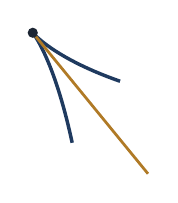
\begin{tikzpicture}
\begin{axis}[width=4.4cm,height=4.4cm,axis lines=none,xmin=-2.12,xmax=-1.6,ymin=-1.4,ymax=0.3,samples=120,smooth]
\addplot[arcetude,domain=-0.7:0.7]({x-2*sqrt(1+x)},{x*ln(1-x)});
\addplot[tgte,samples=2,domain=0:0.27]({-2+x},{-4*x});
\node[pt] at (axis cs:-2,0) {};
\end{axis}
\end{tikzpicture}
\end{columns}
\end{frame}

\begin{frame}{Inflexion : d'où vient $\det(f',f'')$ ?}
Pour un graphe $y=g(x)$ : la courbe est au-dessus de ses tangentes si $g''>0$, au-dessous si $g''<0$.
\pause
Près d'un point régulier où $x'\neq0$ : $y(t)=g\big(x(t)\big)$. On dérive deux fois :
\[y'=g'(x)\,x',\qquad y''=g''(x)\,x'^2+g'(x)\,x''.\]
\pause
On élimine $g'(x)=\frac{y'}{x'}$ :
\[\boxed{\ g''\big(x(t)\big)=\frac{x'y''-y'x''}{x'^3}=\frac{\det(f',f'')}{x'^3}\ }\]
\pause
\begin{columns}[c]
\column{0.55\textwidth}
$x'^3$ garde un signe près de $t_0$ : \textbf{le signe de $\det(f',f'')$ dit de quel côté de ses tangentes est la courbe.}
\column{0.4\textwidth}\centering\onslide<1->
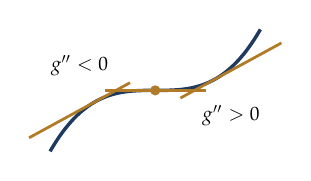
\begin{tikzpicture}
\begin{axis}[width=5cm,height=3.3cm,axis lines=none,xmin=-1.6,xmax=1.6,ymin=-1.3,ymax=1.3,samples=100]
\addplot[arcetude,domain=-1.25:1.25]{0.6*x^3};
\addplot[tgte,domain=-1.5:-0.3,samples=2]{0.6*(-0.343)+1.8*0.49*(x+0.7)};
\addplot[tgte,domain=0.3:1.5,samples=2]{0.6*0.343+1.8*0.49*(x-0.7)};
\addplot[tgte,domain=-0.6:0.6,samples=2]{0};
\node[font=\scriptsize,anchor=south] at (axis cs:-0.9,0.1) {$g''<0$};
\node[font=\scriptsize,anchor=north] at (axis cs:0.9,-0.1) {$g''>0$};
\node[pt,fill=Ocre] at (axis cs:0,0) {};
\end{axis}
\end{tikzpicture}
\end{columns}
\end{frame}

\begin{frame}{Inflexion : les conséquences}
\begin{FORM}[Inflexion et $\det(f',f'')$]
\begin{itemize}
\item Inflexion (point régulier) $\iff\det(f',f'')$ \textbf{change de signe}. Nécessaire : $\det=0$.
\item Birégulier ($\det\neq0$) : point ordinaire, courbe du côté de $f''$.
\item Pente : $p'=\dfrac{\det(f',f'')}{x'^2}$ $\Rightarrow$ pente \textbf{extrémale} à l'inflexion (racine double de $p(t)=m$).
\item Si $x'=0$ : $x=h(y)$, $h''=-\dfrac{\det(f',f'')}{y'^3}$.
\end{itemize}
\end{FORM}
\end{frame}

\begin{frame}{Piège : colinéarité, pas annulation}
\begin{PIEGE}
C'est la \textbf{colinéarité} $f''\parallel f'$ qui compte, pas $f''=\ve0$.
\end{PIEGE}
\begin{columns}[T]
\column{0.48\textwidth}\centering
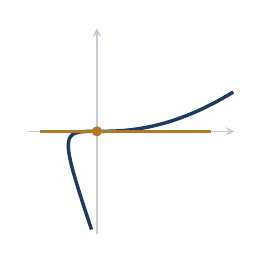
\begin{tikzpicture}
\begin{axis}[mini,width=4.2cm,height=4.2cm,xmin=-0.6,xmax=1.2,ymin=-0.9,ymax=0.9]
\addplot[arcetude,domain=-0.95:0.7]({x+x^2},{x^3});\draw[tgte](axis cs:-0.5,0)--(axis cs:1,0);\node[pt,fill=Ocre] at (axis cs:0,0){};
\end{axis}
\end{tikzpicture}\\
$(t+t^2,t^3)$ : $f''(0)=(2,0)\neq\ve0$,\\ $\det=6t(t+1)$ \textbf{change de signe} :\\ \rep{inflexion}.
\column{0.48\textwidth}\centering
\pause
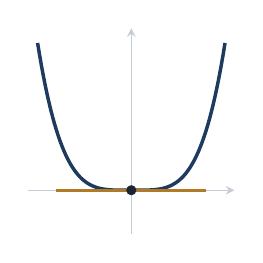
\begin{tikzpicture}
\begin{axis}[mini,width=4.2cm,height=4.2cm,xmin=-1.1,xmax=1.1,ymin=-0.3,ymax=1.1]
\addplot[arcetude,domain=-1:1]({x},{x^4});\draw[tgte](axis cs:-0.8,0)--(axis cs:0.8,0);\node[pt] at (axis cs:0,0){};
\end{axis}
\end{tikzpicture}\\
$(t,t^4)$ : $f''(0)=\ve0$,\\ $\det=12t^2\geq0$ : \rep{pas d'inflexion}.
\end{columns}
\end{frame}

\begin{frame}{Méthode : chercher les inflexions}
\begin{METH}{Chercher les inflexions}
\begin{enumerate}
\item \textbf{Factoriser la vitesse} : $f'=\lambda\ve g$, $\lambda$ scalaire $\neq0$ $\Rightarrow\det(f',f'')=\lambda^2\det(\ve g,\ve g')$.
\item Résoudre $\det(\ve g,\ve g')=0$ aux points réguliers ; trigonométrique : linéariser.
\item Confirmer : changement de signe, ou $\det(f',f''')\neq0$ ($q=3$). Stationnaires : par DL ($p,q$ impairs).
\end{enumerate}
\end{METH}
\pause
\textbf{Pourquoi factoriser ?} \ $f''=\lambda'\ve g+\lambda\ve g'$, donc
\[\det(f',f'')=\det(\lambda\ve g,\lambda'\ve g+\lambda\ve g')=\lambda\lambda'\underbrace{\det(\ve g,\ve g)}_{0}+\lambda^2\det(\ve g,\ve g').\]
\pause
{\small Trigonométrique : factoriser par l'angle moitié, $\cos t-\cos2t=2\sin\frac t2\sin\frac{3t}2$ (§2.1).}
\end{frame}

% =====================================================================
\partie{2.5}{Branches infinies, positions}{Quand le point part à l'infini, la courbe s'approche-t-elle d'une droite ?}{\rmII}

\begin{frame}{Asymptote : définition et critère}
\begin{DEF}
$\|\vv{OM(t)}\|\to\infty$ quand $t\to t_0$ : $\mathcal D$ est \textbf{asymptote} si $d\big(M(t),\mathcal D\big)\to0$.
\end{DEF}
\begin{FORM}[Distance point--droite]
\[d\big(M_0,\ ax+by+c=0\big)=\frac{|ax_0+by_0+c|}{\sqrt{a^2+b^2}}.\]
\end{FORM}
\pause
Pour $\mathcal D:y=\alpha x+\beta$ :\quad $d\to0\iff y-\alpha x\to\beta$.\quad En divisant par $x$ : $\frac yx\to\alpha$.
\pause
\begin{RETENIR}
D'abord $\lim\frac yx=\alpha$ (la \emph{direction}), \textbf{puis} $\lim(y-\alpha x)=\beta$ (la \emph{position} de la droite).
La première limite seule ne prouve rien.
\end{RETENIR}
\end{frame}

\begin{frame}{Classer une branche infinie}
\begin{center}
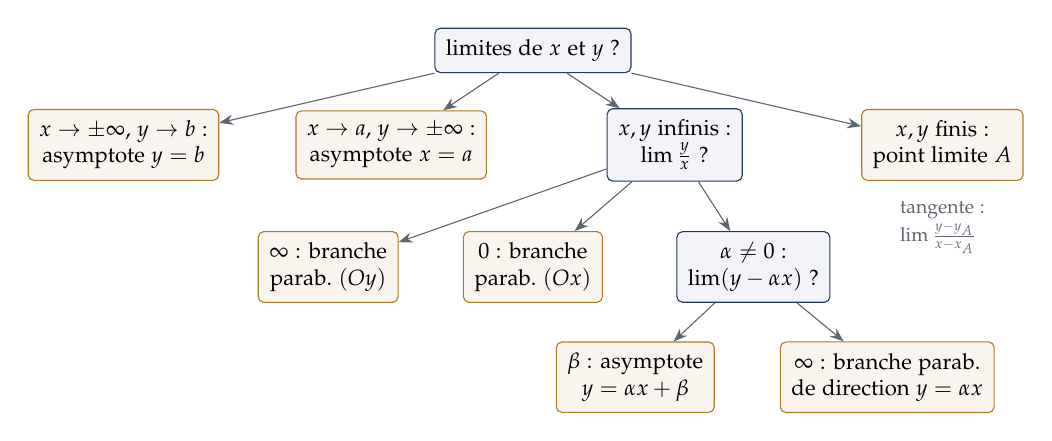
\begin{tikzpicture}[font=\footnotesize,
  q/.style={rectangle,rounded corners=2pt,draw=Bleu,fill=Fond,align=center,inner sep=4pt},
  r/.style={rectangle,rounded corners=2pt,draw=Ocre,fill=Ocre!8,align=center,inner sep=4pt},
  l/.style={font=\scriptsize,Gris}, ->]
\node[q] (a) at (0,0) {limites de $x$ et $y$ ?};
\node[r] (h) at (-5.2,-1.2) {$x\to\pm\infty$, $y\to b$ :\\ asymptote $y=b$};
\node[r] (v) at (-1.8,-1.2) {$x\to a$, $y\to\pm\infty$ :\\ asymptote $x=a$};
\node[q] (b) at (1.8,-1.2) {$x,y$ infinis :\\ $\lim\frac yx$ ?};
\node[r] (pl) at (5.2,-1.2) {$x,y$ finis :\\ point limite $A$};
\draw[Gris] (a)--(h); \draw[Gris] (a)--(v); \draw[Gris] (a)--(b); \draw[Gris] (a)--(pl);
\node[r] (oy) at (-2.6,-2.75) {$\infty$ : branche\\ parab.\ $(Oy)$};
\node[r] (ox) at (0,-2.75) {$0$ : branche\\ parab.\ $(Ox)$};
\node[q] (c) at (2.8,-2.75) {$\alpha\neq0$ :\\ $\lim(y-\alpha x)$ ?};
\draw[Gris] (b)--(oy); \draw[Gris] (b)--(ox); \draw[Gris] (b)--(c);
\node[r] (as) at (1.3,-4.15) {$\beta$ : asymptote\\ $y=\alpha x+\beta$};
\node[r] (bp) at (4.5,-4.15) {$\infty$ : branche parab.\\ de direction $y=\alpha x$};
\draw[Gris] (c)--(as); \draw[Gris] (c)--(bp);
\node[l,align=left,anchor=north] at (5.2,-1.8) {tangente :\\ $\lim\frac{y-y_A}{x-x_A}$};
\end{tikzpicture}
\end{center}
\vspace{-0.15cm}
{\small Pour \textbf{chaque} borne et valeur interdite. Position : signe de $y-\alpha x-\beta$ (développement asymptotique).}
\end{frame}

% ---------------------------------------------------------------- EXERCICE C4
\begin{frame}{\badgeexo{8}Une branche infinie}
\begin{ENONCE}[6 min]
Soit $f(t)=\left(\dfrac t{t-1},\ \dfrac{t^2}{t-1}\right)$. Étudier la branche infinie quand $t\to1$ : direction asymptotique,
asymptote éventuelle, position de la courbe.
\objectif{$\frac yx$, puis $y-\alpha x$, puis le signe de l'écart.}
\end{ENONCE}
\end{frame}

\begin{frame}{\badgecor{8}Une branche infinie}
\begin{columns}[T]
\column{0.38\textwidth}
\begin{RAIS}
$x$ et $y$ tendent vers l'infini : on cherche la pente $\alpha=\lim\frac yx$, puis $\lim(y-\alpha x)$.
\end{RAIS}
\begin{OUTIL}
Classification des branches infinies (§2.5).
\end{OUTIL}
\column{0.59\textwidth}
\etape{1.} $\frac yx=t\to1$ : direction asymptotique de pente $1$.\\[3pt]
\pause
\etape{2.} $y-x=\frac{t^2-t}{t-1}=t\to1$ : \textbf{asymptote} $y=x+1$.\\[3pt]
\pause
\etape{3.} $y-(x+1)=t-1$ : la courbe est au-dessus de l'asymptote pour $t>1$, en dessous pour $t<1$.
\end{columns}
\end{frame}

\begin{frame}{Exemple : une asymptote oblique \ajout}
\[x(t)=t+\frac1{t-1},\qquad y(t)=t^2+\frac2{t-1},\qquad t\neq1.\]
\begin{columns}[c]
\column{0.58\textwidth}
\pause
\textbf{$t\to1$ :} $x,y\to\infty$ ; $\dfrac yx=\dfrac{t^2(t-1)+2}{t(t-1)+1}\to2$.
\pause\par\smallskip
$y-2x=t^2-2t\to-1$ : \textbf{asymptote} $y=2x-1$.
\pause\par\smallskip
Position : $y-2x+1=t^2-2t+1=(t-1)^2>0$ : \rep{courbe au-dessus}, des deux côtés.
\pause\par\smallskip
\textbf{$t\to\pm\infty$ :} $x\sim t$, $y\sim t^2$, $\frac yx\to\pm\infty$ : branche parabolique de direction $(Oy)$.
\column{0.4\textwidth}\centering\onslide<1->
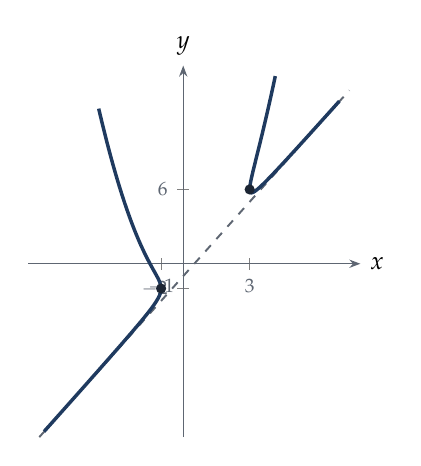
\begin{tikzpicture}
\begin{axis}[courbe,width=5.8cm,height=6.3cm,axis equal image=false,xmin=-7,xmax=8,ymin=-14,ymax=16,xtick={-1,3},ytick={-2,6},
  restrict y to domain=-14:16,restrict x to domain=-7:8]
\addplot[asy,domain=-6.5:7.5,samples=2]{2*x-1};
\only<2->{\addplot[arcetude,domain=-3.6:0.86,samples=300]({x+1/(x-1)},{x^2+2/(x-1)});
\addplot[arcetude,domain=1.17:3.8,samples=300]({x+1/(x-1)},{x^2+2/(x-1)});
\node[pt] at (axis cs:-1,-2) {}; \node[pt] at (axis cs:3,6) {};}
\end{axis}
\end{tikzpicture}
\end{columns}
\end{frame}

\begin{frame}{Position globale par rapport à une droite}
\begin{METH}{Position globale}
$\varphi(t)=ax(t)+by(t)+c$ :
\begin{itemize}
\item zéros de $\varphi$ = points d'intersection avec $ax+by+c=0$ ;
\item signe de $\varphi$ = côté ($b<0$ : $\varphi>0$ signifie au-dessous) ;
\item tangente en $M(t_0)$ : $t_0$ racine \textbf{double} de $\varphi$, donc $(t-t_0)$ facteur de $\varphi'$.
\end{itemize}
\end{METH}
\pause
Dans l'exemple : $\varphi(t)=y-2x+1=(t-1)^2$ ne s'annule jamais pour $t\neq1$ : la courbe ne coupe pas son asymptote.
\pause
\begin{PIEGE}[Pièges]
Oublier une borne du domaine. Factoriser le dénominateur ($1+t^3=(1+t)(1-t+t^2)$) avant de calculer $y-\alpha x$.
Un carré au numérateur de $y-\alpha x-\beta$ : même côté des deux côtés.
\end{PIEGE}
\end{frame}

\begin{frame}{Point limite ; pour aller plus loin \HP}
\textbf{Limites finies :} $M(t)\to A$. On place $A$ (cercle creux s'il n'est pas atteint) ; la tangente est la limite de la
corde : $\lim\frac{y-y_A}{x-x_A}$. Si $A=O$ : c'est $\lim\frac yx$ (la corde issue de $O$ tend vers la tangente).
\pause
\begin{HPBOX}
\textbf{Courbe asymptote} $\Gamma$ : exhiber $P_t\in\Gamma$ avec $M(t)P_t\to0$. Même abscisse : $y-g(x)\to0$ (parabole :
$y-\frac{x^2}2\to0$). Pour une exponentielle, à même ordonnée, $x-\ln(y-c)\to0$ est vrai pour \emph{toute} constante $c$ ;
seule la distance verticale en privilégie une.\\[2pt]
\textbf{Polaires} : $x=r\cos\theta$, $y=r\sin\theta$, partir de $x^2+y^2=r^2$. Cardioïde $r=1-\cos\theta$ ;
lemniscate $(x^2+y^2)^2=xy$, $r^2=\frac12\sin2\theta$.
\end{HPBOX}
\end{frame}

% =====================================================================
\partie{2.6}{Intersections, points doubles}{Comment trouver les points où la courbe se recoupe, ou recoupe une droite ?}{\rmII}

\begin{frame}{Deux méthodes}
\begin{METH}{Intersection courbe/droite}
Substituer $x(t)$, $y(t)$ dans l'équation de la droite. Trigonométrique : tout en $X=\cos t$, élever au carré
($\sin^2t=1-X^2$), factoriser ; \textbf{vérifier les signes} à la fin. Tangence : racine double.
\end{METH}
\pause
\begin{METH}{Points doubles}
Résoudre $f(t)=f(s)$, $t\neq s$ ; une symétrie aide (point de l'axe $(Oy)$ : $x(t)=0$).\\
Sans formule (tableau) : écrire deux arcs comme graphes et appliquer le TVI à $h_1-h_2$ (TD 1).\\
Tangentes au point double : une par paramètre.
\end{METH}
\pause
\textbf{Synthèse :} on applique tout le chapitre à une courbe de Lissajous.
\end{frame}

\begin{frame}{Synthèse : $f(t)=(\cos3t,\ 2\sin t)$ --- réduction}
\begin{columns}[c]
\column{0.56\textwidth}
\begin{itemize}
\item $2\pi$-périodique ; $f(-t)=(x,-y)$ : axe $(Ox)$ ;\\ $f(\pi-t)=(-x,y)$ : axe $(Oy)$.\\
      Étude sur $\big[0,\frac\pi2\big]$.
\pause
\item $x'=-3\sin3t$ (nul en $0$, $\frac\pi3$), $y'=2\cos t>0$ sauf en $\frac\pi2$ : courbe \textbf{régulière}.
\pause
\item $x$ : $1\searrow-1$ ($t=\frac\pi3$) $\nearrow0$ ; \ $y$ : $0\nearrow2$.
\item Tangentes verticales en $(1,0)$ et $(-1,\sqrt3)$, horizontale en $(0,2)$.
\end{itemize}
\column{0.4\textwidth}\centering\onslide<1->
\begin{tikzpicture}
\begin{axis}[courbe,width=4.6cm,height=7cm,xmin=-1.35,xmax=1.35,ymin=-2.3,ymax=2.3,xtick={-1,1},ytick={-2,2}]
\only<3->{\addplot[reste,domain=0:6.2832,samples=400]({cos(3*x)},{2*sin(x)});}
\only<2->{\addplot[arcetude,domain=0:1.5708,samples=200]({cos(3*x)},{2*sin(x)});}
\end{axis}
\end{tikzpicture}
\end{columns}
\end{frame}

\begin{frame}{Synthèse --- point double et tangentes}
\begin{columns}[c]
\column{0.56\textwidth}
\begin{ATOI}
$x(t)=0$ et $y(t)=1$ : pour quels $t\in[0,\pi]$ ?
\end{ATOI}
\pause
$\sin t=\frac12$ : $t=\frac\pi6$ ou $\frac{5\pi}6$, et $\cos3t=0$ dans les deux cas : \rep{point double $J=(0,1)$}.
\pause
\[f'\big(\tfrac\pi6\big)=(-3,\sqrt3),\qquad f'\big(\tfrac{5\pi}6\big)=(-3,-\sqrt3).\]
\pause
\[T_1:\ y=-\frac x{\sqrt3}+1,\qquad T_2:\ y=\frac x{\sqrt3}+1.\]
\column{0.4\textwidth}\centering\onslide<1->
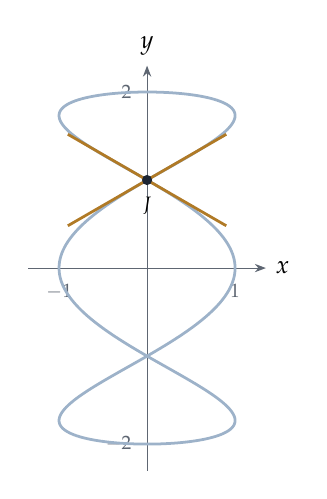
\begin{tikzpicture}
\begin{axis}[courbe,width=4.6cm,height=7cm,xmin=-1.35,xmax=1.35,ymin=-2.3,ymax=2.3,xtick={-1,1},ytick={-2,2}]
\addplot[reste,domain=0:6.2832,samples=400]({cos(3*x)},{2*sin(x)});
\only<4->{\addplot[tgte,domain=-0.9:0.9,samples=2]{-x/sqrt(3)+1};
\addplot[tgte,domain=-0.9:0.9,samples=2]{x/sqrt(3)+1};}
\node[pt] at (axis cs:0,1) {}; \node[font=\scriptsize,anchor=north] at (axis cs:0,0.92) {$J$};
\end{axis}
\end{tikzpicture}
\end{columns}
\end{frame}

\begin{frame}{Synthèse --- où $T_2$ recoupe-t-elle la courbe ?}
$M(t)\in T_2\iff2\sin t=\frac{\cos3t}{\sqrt3}+1$. \ On pose $X=\cos t$, $\cos3t=4X^3-3X$ :\ \ $2\sqrt3\sin t=4X^3-3X+\sqrt3$.
\pause
\par\smallskip
On élève au carré ($\sin^2t=1-X^2$) :
\begin{align*}P(X)&=(4X^3-3X+\sqrt3)^2-12(1-X^2)\\&=16\Big(X-\tfrac{\sqrt3}2\Big)\Big(X+\tfrac{\sqrt3}2\Big)^2\Big(X^3-\tfrac{\sqrt3}2X^2+\tfrac{\sqrt3}2\Big).\end{align*}
\pause
\begin{itemize}
\item $X=-\frac{\sqrt3}2$, \textbf{racine double} : la tangence ($t=\frac{5\pi}6$) ;\ \ $X=\frac{\sqrt3}2$ : l'autre branche par $J$.
\item Dernier facteur : une racine réelle $X_0\approx-0{,}735$.
\end{itemize}
\pause
\begin{PIEGE}[Vérifier le signe (élévation au carré)]
$\sin t=\frac{4X_0^3-3X_0+\sqrt3}{2\sqrt3}\approx0{,}68>0$ : convient. \ Un seul autre point : $K\approx(0{,}62\,;\,1{,}36)$.
\end{PIEGE}
\end{frame}

\begin{frame}{Synthèse --- inflexions}
\begin{columns}[c]
\column{0.58\textwidth}
\[\det(f',f'')=\dt{-3\sin3t&-9\cos3t\\2\cos t&-2\sin t}\]\[=6(\sin3t\sin t+3\cos3t\cos t).\]
\pause
\textbf{Linéariser} (plus court que $\tan$) :
\[\det=12\cos2t+6\cos4t=6(2c^2+2c-1)\]
avec $c=\cos2t$ (car $\cos4t=2c^2-1$).
\pause
Nul pour $c=\frac{\sqrt3-1}2$ : sur $\big[0,\frac\pi2\big]$, seul $\alpha\approx0{,}598$, où $\det$ \textbf{change de signe}.
\pause
\begin{RETENIR}
$M(\alpha)\approx(-0{,}22\,;\,1{,}13)$ est une inflexion ; par symétrie, \textbf{quatre} inflexions.
\end{RETENIR}
\column{0.38\textwidth}\centering\onslide<1->
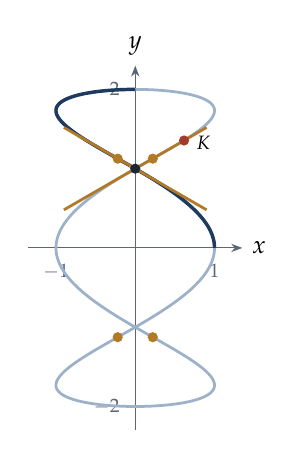
\begin{tikzpicture}
\begin{axis}[courbe,width=4.3cm,height=6.4cm,xmin=-1.35,xmax=1.35,ymin=-2.3,ymax=2.3,xtick={-1,1},ytick={-2,2}]
\addplot[reste,domain=0:6.2832,samples=400]({cos(3*x)},{2*sin(x)});
\addplot[arcetude,domain=0:1.5708,samples=200]({cos(3*x)},{2*sin(x)});
\addplot[tgte,domain=-0.9:0.9,samples=2]{-x/sqrt(3)+1};
\addplot[tgte,domain=-0.9:0.9,samples=2]{x/sqrt(3)+1};
\node[pt] at (axis cs:0,1) {};
\node[pt,fill=Brique] at (axis cs:0.6154,1.3553) {}; \node[font=\scriptsize,anchor=west] at (axis cs:0.65,1.33) {$K$};
\only<4->{\node[pt,fill=Ocre] at (axis cs:-0.2214,1.126) {}; \node[pt,fill=Ocre] at (axis cs:0.2214,1.126) {};
\node[pt,fill=Ocre] at (axis cs:-0.2214,-1.126) {}; \node[pt,fill=Ocre] at (axis cs:0.2214,-1.126) {};}
\end{axis}
\end{tikzpicture}
\end{columns}
\end{frame}

% =====================================================================
\partie{2.7}{Check-list et résultats des TD}{Avant de rendre une étude de courbe : ai-je tout vérifié ?}{\rmII}

\begin{frame}{La check-list d'une étude}
\begin{columns}[T]
\column{0.5\textwidth}
\begin{enumerate}
\item Domaine, valeurs interdites ; symétries \textbf{vérifiées}.
\item Dérivées \textbf{factorisées} ; zéros communs.
\item Tangentes : régularité vérifiée.
\item DL jusqu'au premier vecteur non colinéaire.
\end{enumerate}
\column{0.48\textwidth}
\begin{enumerate}\setcounter{enumi}{4}
\item \textbf{Toutes} les branches ; $\lim(y-\alpha x)$ ; position.
\item Position globale : $\varphi$ ; inflexions : $\lambda\ve g$.
\item Élévation au carré : signes.
\item Tracé fidèle (positions, tangentes, symétries).
\end{enumerate}
\end{columns}
\pause
\begin{RETENIR}
\begin{itemize}
\item Tangente : $M(t_0)+\vect f'(t_0)$ si régulier ; sinon le premier vecteur non nul du DL.
\item Nature locale : parités de $(p,q)$. \quad Concavité : signe de $\det(f',f'')$.
\item Asymptote : $\lim\frac yx$, \textbf{puis} $\lim(y-\alpha x)$, puis position.
\end{itemize}
\end{RETENIR}
\pause
\textbf{Au travail :} TD 1 à 10 de courbes, avec la fiche (§2.7 : résultats des TD pour se corriger).
\end{frame}

\begin{frame}[plain]
\begin{tikzpicture}[remember picture,overlay]
  \fill[Bleu] (current page.north west) rectangle (current page.south east);
  \node[anchor=north west,text=white,font=\sffamily\bfseries\LARGE] at ([xshift=1cm,yshift=-1.4cm]current page.north west) {Après la séance};
  \node[anchor=north west,text width=13.5cm,text=white,font=\normalsize] at ([xshift=1cm,yshift=-2.6cm]current page.north west)
   {\color{white}\setbeamercolor{normal text}{fg=white}\usebeamercolor[fg]{normal text}\begin{itemize}\itemsep6pt
    \item[\textcolor{Ocre}{\rule{0.4em}{0.4em}}] La \textbf{fiche} reprend chaque partie sous le même numéro (§1.1 à §2.7), avec les mêmes notations.
    \item[\textcolor{Ocre}{\rule{0.4em}{0.4em}}] Réviser : relire la fiche, refaire les exemples des diapositives sans regarder la solution.
    \item[\textcolor{Ocre}{\rule{0.4em}{0.4em}}] S'entraîner : TD, puis problème type devoir du livre en 1\,h\,30.
    \item[\textcolor{Ocre}{\rule{0.4em}{0.4em}}] Se corriger : résultats des TD en fin de chaque chapitre de la fiche.
   \end{itemize}};
\end{tikzpicture}
\end{frame}


\end{document}
